
\subsection{Features of the BGT60TR13C}

Figure \ref{fig:BGT60TR13CBoard} shows a diagram of the DEMO BGT60TR13C TOBO1 development board (2), which includes a radar shield (5) with a BGT60TR13C radar chip (4), and a microcontroller (3) to convert data from the radar chip by the SPI protocol and transmit to external devices via USB.

\begin{figure}[H]
    \centering
    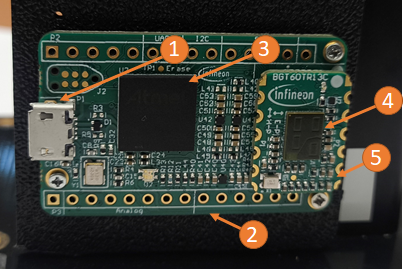
\includegraphics[width=0.5\linewidth]{Src/images/BGTdevBoard.png}
    \caption{DEMO BGT60TR13C TOBO1 Board}
    \label{fig:BGT60TR13CBoard}
\end{figure}

The direction of data flows is shown in the figure \ref{fig:Data Flow diagram}. This radar chip performs only preliminary signal processing, such as built-in ADC, and allows only to configure emission and digitisation parameters tuning via memory registers such as frequency, bandwidth, duration, and number of samples (chirps). Data processing takes place only on the application processor, which was a personal computer or a single-board computer such as Raspberry PI.






\begin{figure}[H]
    \centering
    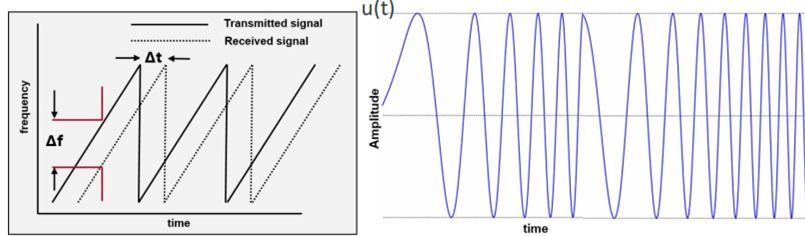
\includegraphics[width=0.85\linewidth]{FMCW.png}
    \caption{FMCW modulation}
    \label{fig:FMCW}
\end{figure}




The module operates based on the frequency-modulated continuous wave (FMCW) principle. As shown in Figure \ref{fig:Radar System block diagram}, the system includes a voltage-controlled oscillator (VCO) that generates a chirp signal—a waveform whose frequency increases linearly over time (Figure \ref{fig:FMCW}). 


\begin{figure}[H]
    \centering
    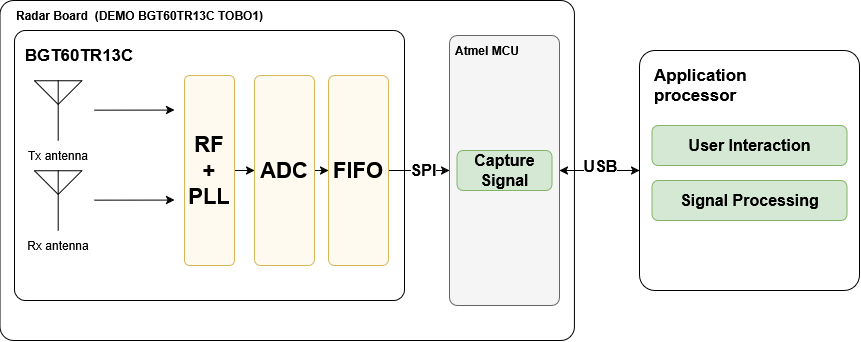
\includegraphics[width=0.7\linewidth]{Src/images/radar board.drawio(1).png}
    \caption{Data Flow diagram}
    \label{fig:Data Flow diagram}
\end{figure}



This signal is subsequently amplified by a power amplifier (PA) and transmitted into free space via a transmit antenna. When the signal reflected signal from the moving robot, it is received by the 1-3 receiving antennas and passed through a low noise amplifier (LNA) for signal conditioning.

\begin{figure}[H]
    \centering
    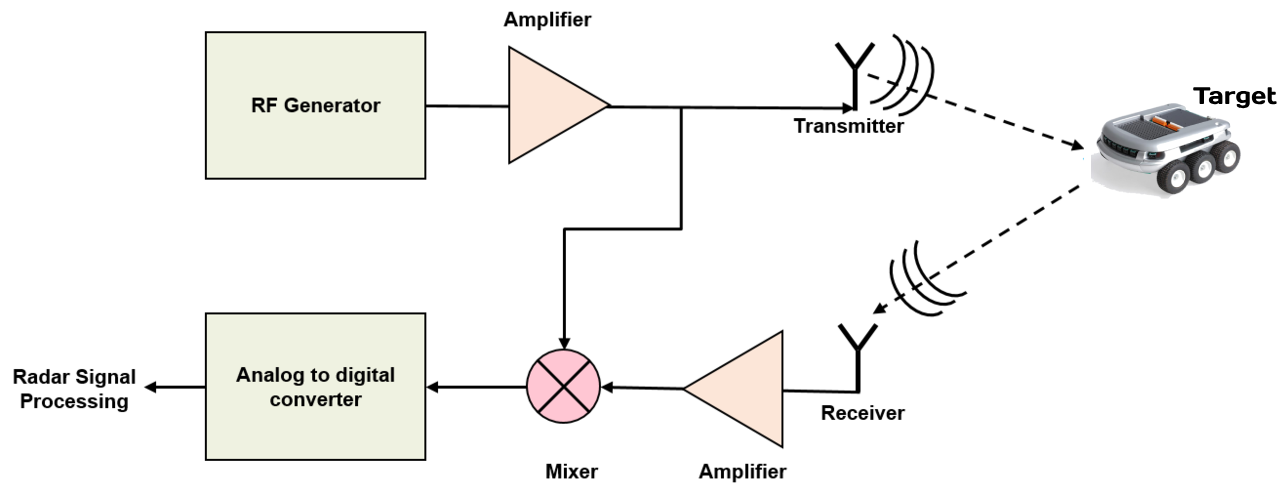
\includegraphics[width=0.9\linewidth]{Src/images/img_typical_radar_system.png}
    \caption{Radar System block diagram}
    \label{fig:Radar System block diagram}
\end{figure}

 The received signal mixed with a copy of the transmitted chirp, resulting in an intermediate frequency (IF) signal, also known as the beat frequency $f_IF$ .This frequency is directly proportional to the time delay between transmission and reception and hence corresponds to the range of the target.
This analogue signal is converted into digital form by ADC and transmitted to an external device for analysis. 

\begin{figure}[H]
    \centering
    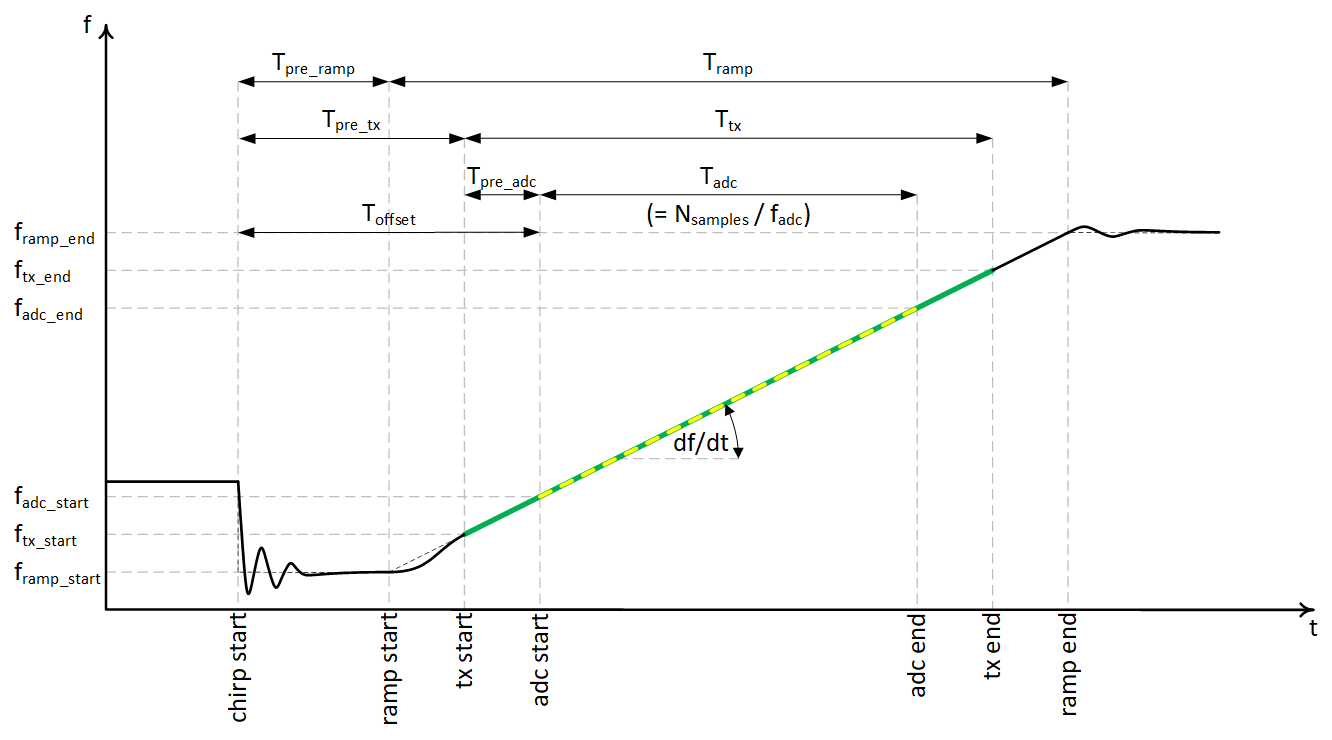
\includegraphics[width=0.85\linewidth]{Src/images/img_chirp_diagram.png}
    \caption{Chirp signal parameters}
    \label{fig:Chirp}
\end{figure}

The parameters of the emitted signal are shown in Figure \ref{fig:Chirp}, where the FMCW signal is described by a chirp.The wave reflected from the target is delayed by $\tau = 2d/c$ ($d$ is the distance to the target, $c$ is the speed of light) and, after mixing with the reference signal, forms an intermediate frequency 
\begin{equation}f_{\text{IF}} = \frac{2 S d}{c},\label{eq:if_freq}
\end{equation}where $B$ is the chirp bandwidth, $T_c$ is its duration, and $S = \frac{B}{T_c}$ is the slope of the linear modulation. The steeper the slope $S$, the higher $f_{\text{IF}}$ for the same distance $d$, which facilitates the measurement of small $d$, but requires a larger bandwidth $B$. The minimum distinguishable distance difference is determined by the chirp bandwidth:
\begin{equation}
\Delta R = \frac{c}{2B}.\label{eq:range_res}
\end{equation}Increasing $B$ linearly improves the resolution $\Delta R$, but increases the spectral requirements and the load on the ADC. At a sampling frequency $F_s$ and slope $S$, the maximum range is estimated by the expression 
\begin{equation}R_{\max} = \frac{F_s\,c}{2S} =\frac{F_s\,c\,T_c}{2B}.\label{eq:max_range}
\end{equation}To increase $R_{\max}$,increase $F_s$ or lengthen $T_c$, but both options reduce the frame rate and increase power consumption.The maximum measurable speed is determined by the chirp repetition period (\textit{Pulse Repetition Time}, PRT):
\begin{equation}
\text{PRT} = \frac{\lambda}{v_{\max}},\label{eq:prt}
\end{equation}
where $f_c$ is the central emission frequency, $\lambda = \frac{c}{f_c}$. Velocity resolution for $N_c$ chirps in a frame
\begin{equation}\Delta v = \frac{2 v_{\max}}{N_c}.\label{eq:vel_res}
\end{equation}Increasing $N_c$ improves $\Delta v$, but proportionally lengthens the frame, which reduces the data refresh rate. For given $R_{\max}$ and $\Delta R$, the required number of samples is determined as
\begin{equation}N_{\text{samples}} = \frac{2 R_{\max}}{\Delta R}. \label{eq:samples} end 
\end{equation}


\begin{table}[H]
\centering
\caption{Comparison of radar configuration parameters}
\label{tab:radar_params}
\begin{tabular}{|l|c|c|c|c|}
\hline
\textbf{Parameter} & \textbf{Config 1} & \textbf{Config 2} & \textbf{Config 3} & \textbf{Config 4} \\
\hline
Samples per Chirp ($N_\text{samples}$) & 64 & 512 & 512 & 512 \\
Range Resolution $\Delta R$ [m] & \textbf{0.028} & 0.078 & 0.078 & \textbf{0.032} \\
Max Range $R_\text{max}$ [m] & 0.9 & \textbf{19.9} & \textbf{19.9} & \textbf{9.1} \\
Chirps per Frame ($N_c$) & 4 & 32 & 32 & 128 \\
Speed Resolution $\Delta V$ [m/s] & \textbf{13.394} & 0.209 & 0.036 & \textbf{0.030} \\
Chirp Repetition Time (PRT) [μs] & 46 & 369 & 210 & 635 \\
Max Speed $v_\text{max}$ [m/s] & \textbf{26.788} & 3.338 & \textbf{0.579} & \textbf{1.994} \\
Frame Rate [Hz] & \textbf{9.69} & 6.96 & 9.96 & \textbf{12.31} \\
Start Frequency $f_\text{start}$ [GHz] & 58.00 & 59.81 & 59.89 & 58.22 \\
End Frequency $f_\text{end}$ [GHz] & 63.38 & 61.74 & 61.73 & 62.96 \\
Bandwidth $d_f$ [GHz] & 5.38 & 1.93 & 1.93 & 4.74 \\
\hline
\end{tabular}
\end{table}


The larger $N_{\text{samples}}$, the higher the range resolution, but the longer the duration of a single chirp $T_c$.Equations (\ref{eq:if_freq})--(\ref{eq:samples}) form a system of interdependencies in which no parameter can be improved in isolation. Table \ref{tab:radar_params} shows the main difference in parameters.

Enclosed spaces High accuracy and update frequency are priorities; it is acceptable to limit $R_{\max}$ to 5–10 m, increasing $B$ and keeping $T_c$ short. 
Open spaces detection range and the range of measurable speeds are important; it is advisable to increase $T_c$ and $N_c$, accepting a lower frame rate.

Thus, the configuration of an FMCW radar for a mobile robot represents a balance between four values: $B$, $T_c$, F$_s$, and the number of chirps $N_c$.



The radar device internally organizes its raw intermediate frequency (IF) samples into a multi-dimensional structure. The dimensions of the like a cube are defined as follows:
\begin{itemize}
    \item \textbf{Rows:} Number of virtual receiving antennas,  the number of physical Rx antennas multiplied by the number of active Tx antennas.
    \item \textbf{Columns:} Number of chirps per frame.
    \item \textbf{Slices:} Number of ADC samples per chirp.
\end{itemize}
    

\begin{figure}[H]
    \centering
    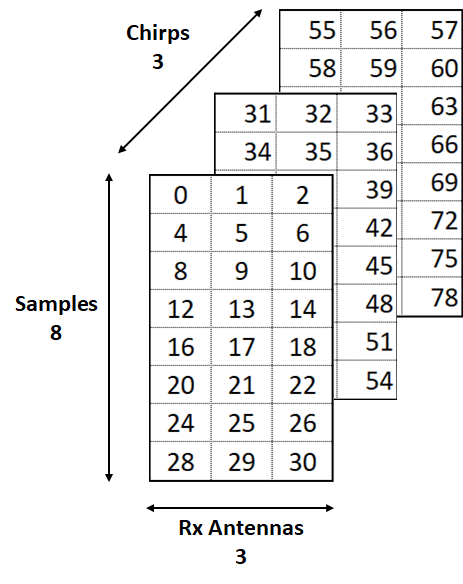
\includegraphics[width=0.4\linewidth]{Src/images/RowData.png}
    \caption{Raw Data representing}
    \label{fig:RadarFrameCube}
\end{figure}

 Each combination of a transmit antenna and a receive antenna defines a virtual channel. The complete radar data for a frame is a concatenation of all such virtual channels over the configured number of chirps and ADC samples.

As illustrated in Figure \ref{fig:RadarFrameCube}, the incoming data is stored sequentially in memory, with rows representing the virtual antenna index, columns representing chirps, and slices representing the ADC samples per chirp.
The total frame contains $8×3×3=72$ complex samples.



\subsection{Signal-to-Noise Ratio  Estimation}

The aim is to evaluate the sensitivity of the radar SNR up to a distance of \SI{5}{m}. These results are necessary to anderstand the losses in the system and also for  selection the detection thresholds. The assumed target is a human body with a radar cross section of \(\sigma = 1\,\si{m^2}\).

\noindent
\textbf{Parapemeters}
\begin{itemize}
    \item Center frequency: \(f_c = \SI{60.75}{GHz}\), FMCW bandwidth: \(B = \SI{1.5}{GHz}\).
    \item Chirp duration: \(\tau = \SI{200}{\micro\second}\), number of chirps per frame: \(N_c = 128\) (frame rate: \SI{20}{Hz}).
    \item Number of samples per chirp: \(N_s = 64\), sample rate: \SI{1}{MHz}.
    \item Active antennas: \(\text{TX}_1\), \(\text{RX}_1\), and \(\text{RX}_3\); antenna gains: \(G_\text{TX} = G_\text{RX} = \SI{5}{dBi}\).
\end{itemize}
\noindent
\textbf{Theoretical SNR Model}
\noindent
The single-chirp SNR is computed using the radar equation \citep{Skolnik2001}:
\begin{equation}
	\label{eq:snr_theor_single}
	\text{SNR}_{\text{1p}}(R)=
	\frac{P_t\,G_\text{TX}G_\text{RX}\,\lambda^{2}\sigma}
	     {(4\pi)^{3} R^{4} k T  B  L_\text{sys}},
\end{equation}
where \(P_t = \SI{10}{dBm}\), \(\lambda = c / f_c\),
\(k = \SI{1.38e-23}{J/K}\), \(T = \SI{290}{K}\),
\(\sigma = \SI{1}{m^{2}}\), and pesumably \(L_\text{sys} = \SI{2}{dB}\).

\noindent
Coherent integration of \(N_c\) pulses adds gain:
\begin{equation}
	G_\text{int}=10\log_{10} N_c,
\qquad
	\text{SNR}_{\text{int}}(R)=\text{SNR}_{\text{1p}}(R)+G_\text{int}.
\end{equation}
\noindent




\begin{figure}[H]
    \centering
    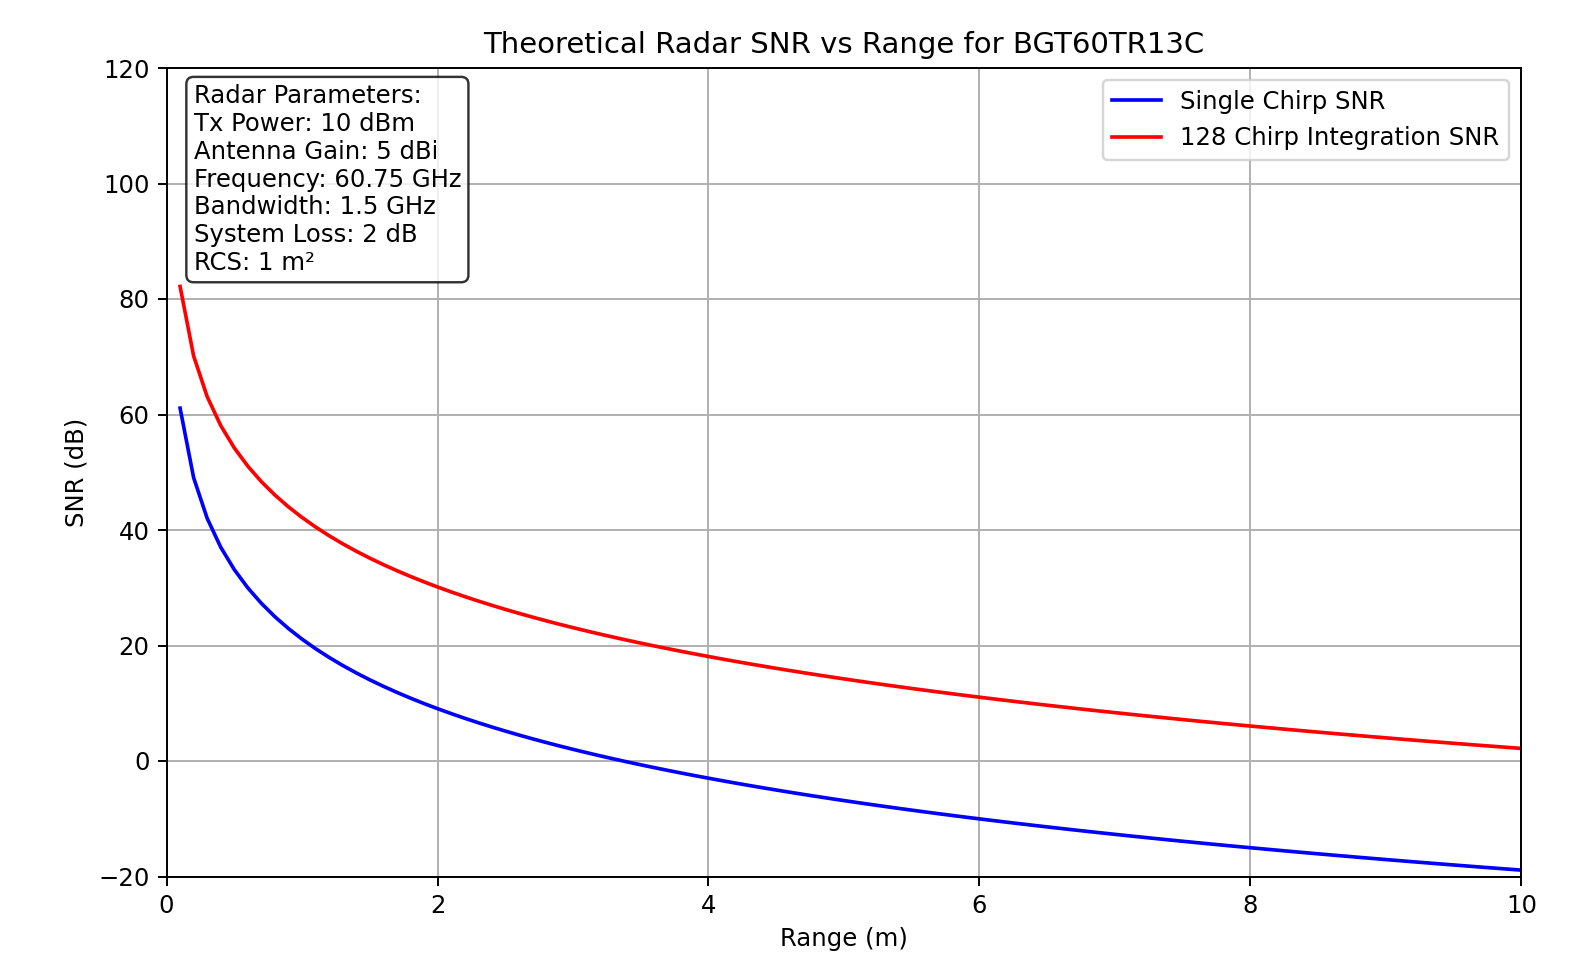
\includegraphics[width=0.7\linewidth]{Src//images/TheoreticalSNR.png}
    \caption{Range–Angle Map, theoretical and measured SNR representation}
    \label{fig:exp4_gui}
\end{figure}



Based on the fundamental radar equation:
$    P_\text{sig} = \frac{P_t\, G_t\, G_r\, \lambda^2\, \sigma}{(4\pi)^3 R^4},
$
and the expression for thermal noise power:
$ P_\text{noise} = k T B L$, the signal-to-noise ratio (SNR) is given by:
$\text{SNR} = \frac{P_\text{sig}}{P_\text{noise}}     \propto R^{-4}$.
With fixed radar parameters for the BGT60TR13C sensor (transmit power $P_t = 10\;\text{mW}$, antenna gains $G_t = G_r = 5\;\text{dBi}$, wavelength $\lambda \approx 4.94\;\text{mm}$, bandwidth $B = 1.5\;\text{GHz}$, temperature $T = 290\;\text{K}$, system losses $L = 10^{2/10}$), the estimated single-chirp SNR values at distances $R = 1\;\text{m}$, $2\;\text{m}$, and $3\;\text{m}$ are approximately 20 dB, 6 dB, and 1 dB, respectively.

Coherent integration of $N = 128$ chirps yields a theoretical gain of:
$    \Delta_\text{int} = 10 \log_{10}(N) \approx 21\;\text{dB},
$
which raises the total SNR to about 41 dB, 27 dB, and 22 dB at the same respective distances.

Considering realistic factors such as variations in human radar cross-section (–3 to –6 dB), multipath fading in indoor environments (–5 to –8 dB), and additional hardware losses (–2 to –3 dB), the combined SNR degradation can reach 10–15 dB. Therefore, at $R \leq 3\;\text{m}$, the integrated SNR remains above the practical detection threshold (typically around 10 dB), even under non-ideal conditions.

Furthermore, limiting the operating range to 3 meters reduces data volume (only 64 range bins with 5 cm resolution), minimizes interference from distant reflectors, and improves the computational load of detection and navigation algorithms in mobile robotic systems.

\subsection{Results of the experiments}


\subsubsection{Detection of Objects with Different Material Properties} 
\noindent
Measure amplitude of peak corresponding to object distance. 
\\
Purpose:
To obtain data from the radar reflectivity and detectability of common materials used in indoor environments. Radio wave interaction with each target differs depending on its dielectric constant, surface roughness, and conductivity.
Procedure:
\begin{itemize}
\item     Place one object at a time at defined distances (1m) in front of the radar
\item     Stream raw complex radar samples to PC
\item     Perform 1D FFT (Equation \ref{eq:range_fft}) to obtain range profiles:

\begin{equation}
    R[m,k] \;=\;
        \sum_{n=0}^{N_s-1} r[n,k]\,
        e^{-j\,2\pi n m / N_s},
    \qquad
    m = 0,\,\dots,\,N_s-1,
    \label{eq:range_fft}
\end{equation}
where $N_s$ is the number of samples per chirp.  \\
The resulting array $R[m,k]$ forms the \emph{range profile}.
\item Transform FFT bin indices to physical distance using (Equation \ref{eq:range_conversion}):
    \begin{equation}
        R[m] = \frac{c \cdot m}{2 \cdot N_s \cdot f_s / B}
        = \frac{c \cdot m \cdot B}{2 \cdot N_s \cdot f_s}
        \label{eq:range_conversion}
    \end{equation}
    where:
    \begin{itemize}
        \item $c$ — speed of light ($\approx 3 \cdot 10^8$ m/s),
        \item $f_s$ — ADC sampling rate,
        \item $B$ — bandwidth of the chirp,
        \item $N_s$ — number of samples per chirp,
        \item $m$ — FFT bin index.
    \end{itemize}
    This converts the horizontal axis of the FFT output to range (in meters), enabling distance estimation for detected reflections.

\end{itemize}
\noindent
Expected Outcome:
Highly conductive materials (steel) should produce strong returns; lossy dielectrics (foam, wood) are expected to result in weaker reflections.

\begin{figure}[H]
    \centering
    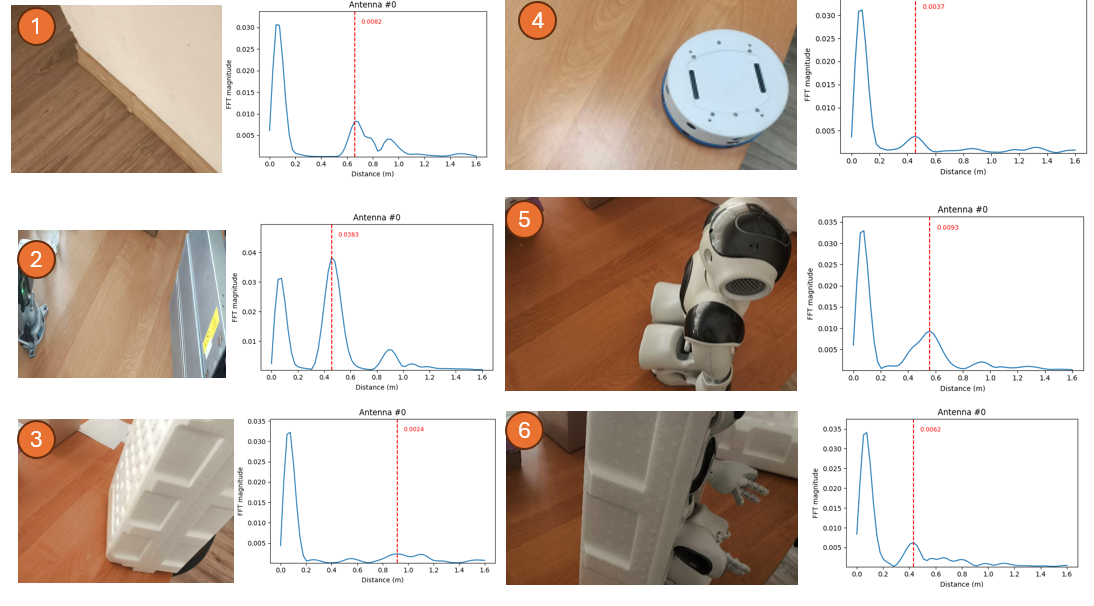
\includegraphics[width=0.85\linewidth]{Src/images/E1S1.png}
    \caption{Object image and Fourier graph for each element}
    \label{fig:Objectvis}
\end{figure}

Figure \ref{fig:Objectvis} provide data of object visibility measured using radar. For each case, the left image shows the target placed at approximately 0.4 to 0.6 m from the radar.The right plot displays the corresponding range FFT output profile from antenna \#0.
Each object is numbered and the following observations were made:
\begin{enumerate}
            \item A wall produces a stable mid-level return.
            \item A metallic wall yields the strongest reflection in the experiment.
            \item A foam box is nearly transparent, with minimal radar return.
            \item The plastic Khepera robot gives a weak signal, barely above noise.
            \item The NAO robot returns a clear peak due to internal metal structures.
            \item When placed inside a foam box, the NAO robot remains detectable, but with attenuated amplitude.
            \item A dry brick produces a moderate return.
            \item A water bottle placed behind the brick creates a stronger second peak, 
            demonstrating the radar's ability to detect to object on different range.
\end{enumerate}

Intresting fact that peak can be seen at a distance from 0 to 0.2 m in almost all experimental recordings, regardless of whether there is an object at this distance.  This may be due to near-field reflections — the signal is reflected from the radar body itself, its antennas, mounting elements or surface. For this reason, the technical specifications specify a minimum detection range of 0.2 m. Below this limit, the reflected signal cannot be interpreted. In further calculations, this part was discarded.

\begin{figure}[H]
    \centering
    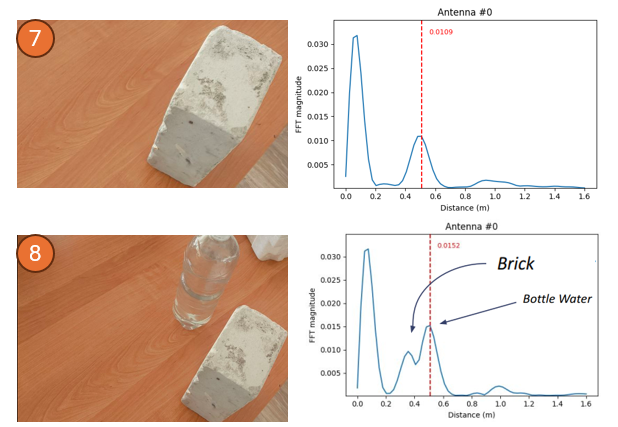
\includegraphics[width=0.6\linewidth]{Src//images/E1S23.png}
    \caption{Object image and Fourier graph for each element}
    \label{fig:Objectvisl2}
\end{figure}

In the Table \ref{tab:material_peaks_clean}, the measured peak reflection amplitudes from various objects of different materials are presented. Materials range from low-loss dielectrics (plastic, wood) to highly reflective or lossy conductors (brick, water bottle) and also on Figure \ref{fig:Objectvisl2}. 


The values are expressed in normalized units ($\times 10^{-3}$) for three parallel channels, designated as Peak A0, A1, and A2. The activation of all three receiving antennas occurred simultaneously, thereby establishing three observation channels for the reflected radar signals.

\begin{table}[H]
\renewcommand{\arraystretch}{0.5} % уменьшение высоты строк
\centering
\small
\caption{Peak detection amplitudes for various materials (values in $\times 10^{-3}$)}
\begin{tabular}{@{}lccccc@{}}
\toprule
\textbf{Material} & $\varepsilon_r$ & \textbf{Distance [m]} & \textbf{Peak A0} & \textbf{Peak A1} & \textbf{Peak A2} \\
\midrule
Battle carton             & 2.3  & 0.43 & 4.8   & 7.0   & 6.5 \\
Battle paper stack        & 3.2  & 0.45 & 8.6   & 12.7  & 10.4 \\
Bottle (water) large      & 80.0 & 0.35 & 8.5   & 8.7   & 8.8 \\
Bottle (water) medium     & 80.0 & 0.38 & 9.7   & \cellcolor{myred}15.4 & 11.5 \\
Bottle (water) small      & 80.0 & 0.40 & \cellcolor{myblue}3.3 & 3.6   & \cellcolor{myblue}5.1 \\
Box (wood)                & 2.4  & 1.00 & 2.4   & 2.9   & \cellcolor{myred}2.6 \\
Brick (dry)               & 4.5  & 0.50 & 10.9  & 17.1  & 13.2 \\
Brick (with water)               & 12.0 & 0.50 & \cellcolor{myred}15.2 & \cellcolor{myred}21.6 & 17.1 \\
Rubber                    & 1.3  & 0.35 & 14.5  & 10.0  & 12.7 \\
Cardboard box  & 2.3  & 0.55 & 8.7   & 12.4  & 11.4 \\
DSP (chipboard)           & 3.5  & 0.45 & 9.7   & 15.4  & 10.9 \\
Hand (human)              & 40.0 & 0.45 & 7.7   & 7.6   & 7.3 \\
Khepera robot (plastic)   & —    & 0.45 & \cellcolor{myblue}3.7 & 4.4   & 5.5 \\
Koala robot (plastic)     & —    & 0.55 & 9.3   & 5.7   & 6.9 \\
NAO box (cardboard)       & —    & 0.45 & 6.2   & 8.3   & 7.7 \\
NAO robot (plastic)       & —    & 0.55 & 9.3   & 14.4  & 12.2 \\
Wall concrete             & 2.5  & 0.65 & 8.2   & 8.5   & 8.2 \\
\bottomrule
\end{tabular}
\label{tab:material_peaks_clean}
\end{table}

As expected, highly reflective materials such as wet brick and rubber produced strong and consistent reflections across all three antennas, with peaks exceeding 0.015. In contrast, low-reflectivity or semi-transparent objects, such as wood, plastic enclosures, and small filled bottles, has lower amplitudes (often below 0.005), sometimes with variability between antennas. In general, using multiple receiving antennas in parallel increases a radar system's spatial diversity.



The results confirm that material composition and spatial scattering characteristics impact the detectability of radar, even at short indoor ranges. Moreover, the magnitude of the reflected signal provides a distinctive signature that can be used not only to estimate the distance to an object, but also to infer its material class or structural properties.


\subsubsection{Influence of Objects and Environmental Conditions on Radar}
\noindent
\textbf{Purpose:}
To investigate how different objects and environmental conditions affect the characteristics of the radar signal. By analyzing signal variations under controlled scenarios, the objective is to understand the impact of object positioning and ambient interference on the features of the BGT60 FMCW radar within a short-range (0 to 3 m) indoor environment.

\paragraph{Radar configuration.}
All experiments below were performed with an Infineon BGT60 FMCW radar using the settings in Table \ref{tab:radar_config}.  
The parameters target a 0–3 m range and 5 cm range resolution; the required bandwidth $B$ follows from $\Delta R = c/(2B)$.

\begin{table}[H]
\centering
\caption{Radar configuration parameters used in the experiment series}
\label{tab:radar_config}
\begin{tabular}{|l|l|l|}
\hline
\textbf{Parameter}           & \textbf{Value} & \textbf{Description} \\
\hline
\texttt{max\_range\_m}       & 5.0 m          & Maximum detection range \\
\texttt{range\_resolution\_m} & 0.05 m         & Range resolution ($\Delta R$ = 5 cm) \\
\texttt{center\_freq}        & 60.75 GHz      & Center frequency \\
\texttt{available\_bandwidth} & 1.5 GHz        & Available bandwidth \\
\texttt{chirp\_time}         & 200 µs         & Chirp duration \\
\texttt{num\_chirps}         & 128            & Number of chirps per frame \\
\texttt{samples\_per\_chirp} & 64             & Number of samples per chirp \\
\texttt{frame\_time}         & 0.2 s          & Frame duration (5 Hz frame rate) \\
\hline
\end{tabular}
\end{table}


\noindent
After digitization the reflected signal is processed by a 1-D FFT (Eq. \ref{eq:range_fft})  
followed by converting the bin index $m$ to physical distance via Eq. \ref{eq:range_conversion}.  
This yields a 5 cm-spaced range profile $R[m,k]$ whose peak amplitudes are analysed below.





\paragraph{Effect of mounting height.}
In this experiment, was explored the impact of the radar's elevation on the output data, considering its broad beam pattern (see Figure \ref{fig:radar-patern}), which leads to reflections from nearby surfaces, particularly the ground.
At the test setup (see Figure \ref{fig:radarstand}), the radar's height was adjusted from 50 mm to 1000 mm in increments of 50 mm, in two scenarios: indoors (on a concrete floor) and outdoors (on asphalt). The radar was positioned perpendicular to the wall at a distance of 2 meters, and the peak values of the signal were recorded and displayed in Figure \ref{fig:radar-flor}.
The findings demonstrated a substantial disparity between indoor and outdoor measurements, primarily attributable to the reflective properties of the floor.
Indoors, the signal is notably stronger, as the concrete floor is highly reflective due to its high dielectric constant. Additionally, there are reflections from the ceiling, which further enhance the signal.

\begin{figure}[H]
    \centering
    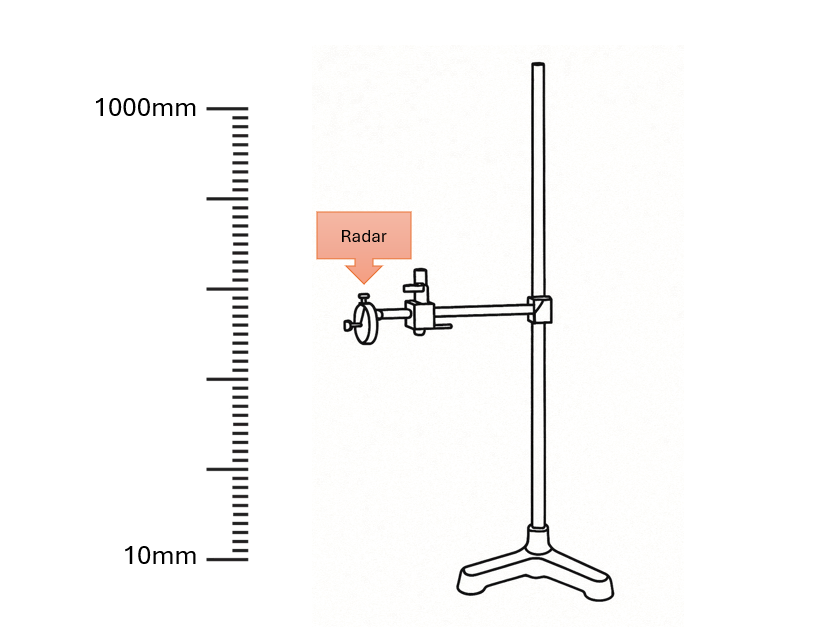
\includegraphics[width=0.5\linewidth]{Src/images/radarstand.png}
    \caption{Radar test stand}
    \label{fig:radarstand}
\end{figure}

On the street, asphalt has a lower dielectric constant and the absence of a ceiling eliminates reflections, reducing the overall signal strength.
At a low radar height, when close to the floor, reflections from the floor, whether it is concrete indoors or asphalt outdoors, become dominant. These strong reflections obstruct the signal from the target object, the wall, causing the signal strength from the wall to decrease significantly.

This is because the wide radiation pattern of the radar captures reflections from the floor, which arrive earlier and have a larger amplitude than the signal from the wall at a distance of two meters.
In the height range between 200 and 400 millimeters, the radar achieves its maximum signal strength from the wall. At this height, the radar is positioned optimally: it is elevated to the influence of its reflections, yet still maintains a strong direct signal from the wall. By increasing the height, the radar can effectively bypass the strong near-field reflections from the floor, resulting in a clearer signal from the wall.

\begin{figure}[H]
        \centering
        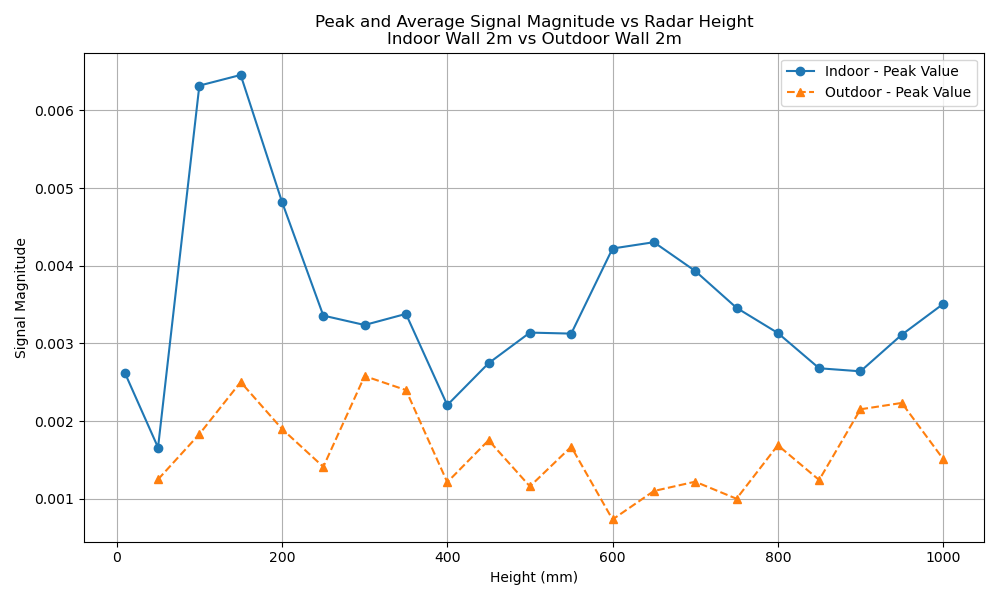
\includegraphics[width=0.75\linewidth]{Src//images/radar flor .png}
        \caption{The influence of floor height on indoor and outdoor spaces}
        \label{fig:radar-flor}
    \end{figure}


However, as the height increases beyond 400 mm, the signal level begins to decrease and stabilizes at a lower value. This is due to two factors: firstly, the length of the direct path to the wall increases (from 2 meters and beyond diagonally), which naturally reduces the signal strength due to signal attenuation. 

\begin{figure}[H]
    \centering
    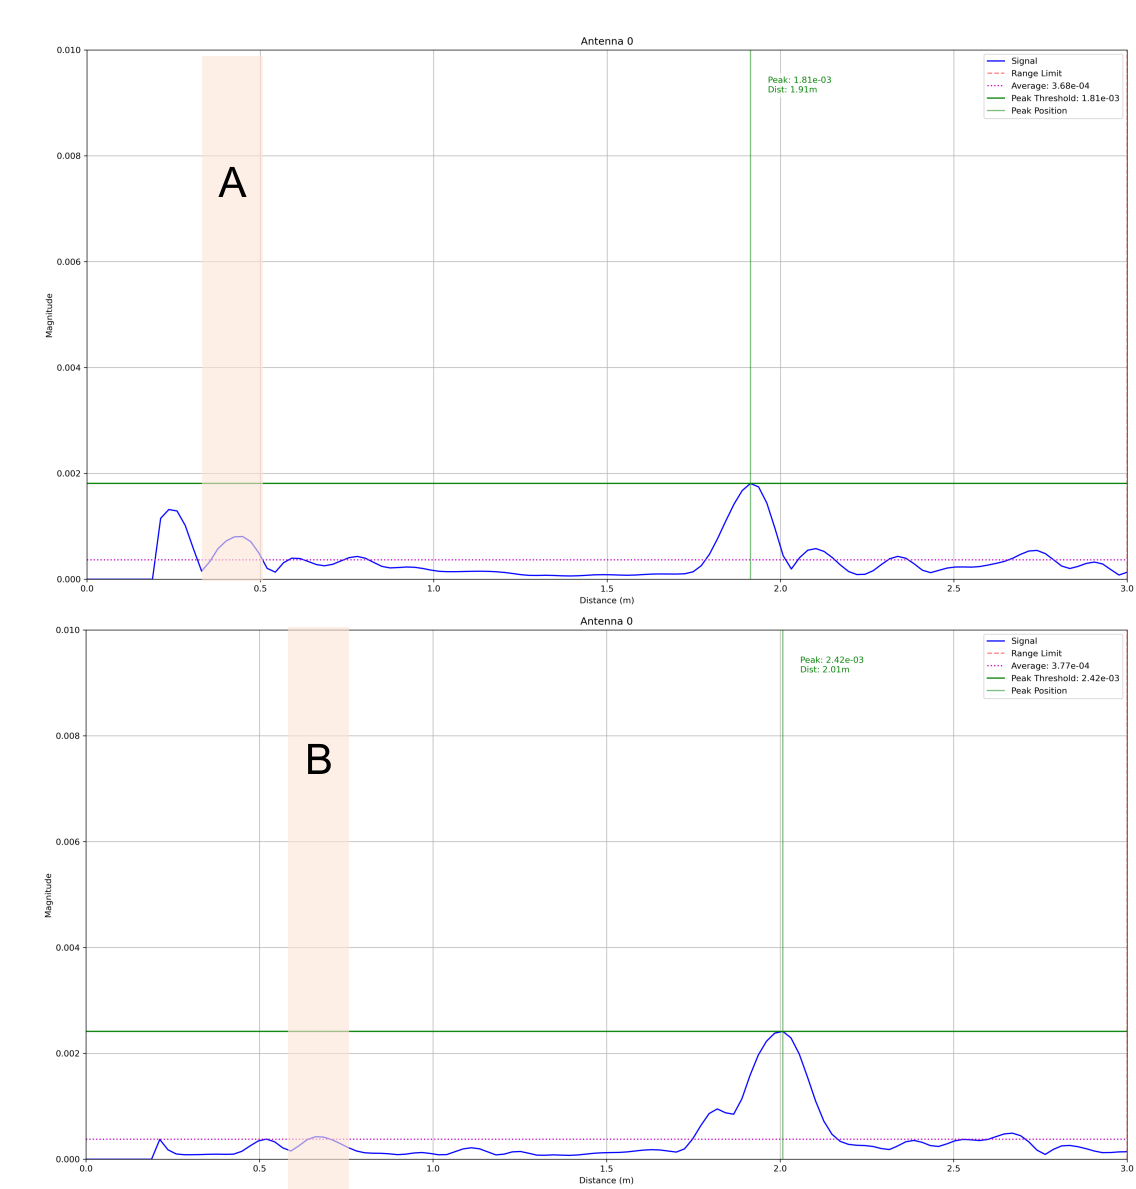
\includegraphics[width=0.7\linewidth]{Src//images/radarreflectionflor2.png}
    \caption{Radar flor reflection on (A) 350 mm and (B) 600mm}
    \label{fig:reflection-flor}
\end{figure}
Secondly, at higher altitudes inside the room, additional reflections from the ceiling start to interfere with the direct signal from the wall. 
In contrast, outdoors, where there is no ceiling, the signal simply weakens due to the greater distance and the reduced intensity of reflections from the asphalt. Consequently, the signal stabilizes as the influence of the floor becomes negligible, and other factors (the length of the path and the absence of additional reflections) maintain it at a constant level.

Additionally, when analyzing the spectrum using the fast Fourier transform (FFT), reflections from the floor can be detected, especially at low installation heights. Figure  \ref{fig:reflection-flor} shows the results, where weak reflected signals are observed in zone A and zone B at a distance approximately equal to the height of the radar above the surface. This is consistent with the expected path of the signal reflected from the floor and received directly without interacting with the target object (wall).

However, the power of reflection from the floor is low compared to the signal, from object especially in open conditions where there are no secondary reflections from the ceiling. Therefore, the analysis of such weak reflections is possible only in static conditions, when the position of the radar and the scene remains unchanged. In dynamic situations (for example, when a robot is moving), reflections from the floor blur in the time domain and are lost against the background of more powerful responses from other objects and noise, which makes them practically unsuitable for reliable interpretation.






\paragraph{Effect of Distance to Walls in a Narrow Corridor}  
This experiment investigated the impact of distance from the wall on radar output data in a confined space, simulating a 1.2 m wide corridor, which corresponds to one of the operational scenarios for a robot (see Figure \ref{fig:radar-wall}, part a). The radar, positioned at a height of approximately 400 mm, with a wide beam pattern in the H-plane (horizontal), generates significant reflections from walls. Figure \ref{fig:radar-wall}, part b, shows a plot of peak signal amplitudes after Fourier transformation, as recorded by the radar.  



\begin{figure}[H]
    \centering
    \begin{minipage}[b]{0.25\linewidth}
        \centering
        \includegraphics[width=\linewidth]{Src/images/Coridor_view.jpg}
        \subcaption{Corridor View}
        \label{fig:corridor-view}
    \end{minipage}
    \begin{minipage}[b]{0.7\linewidth}
        \centering
        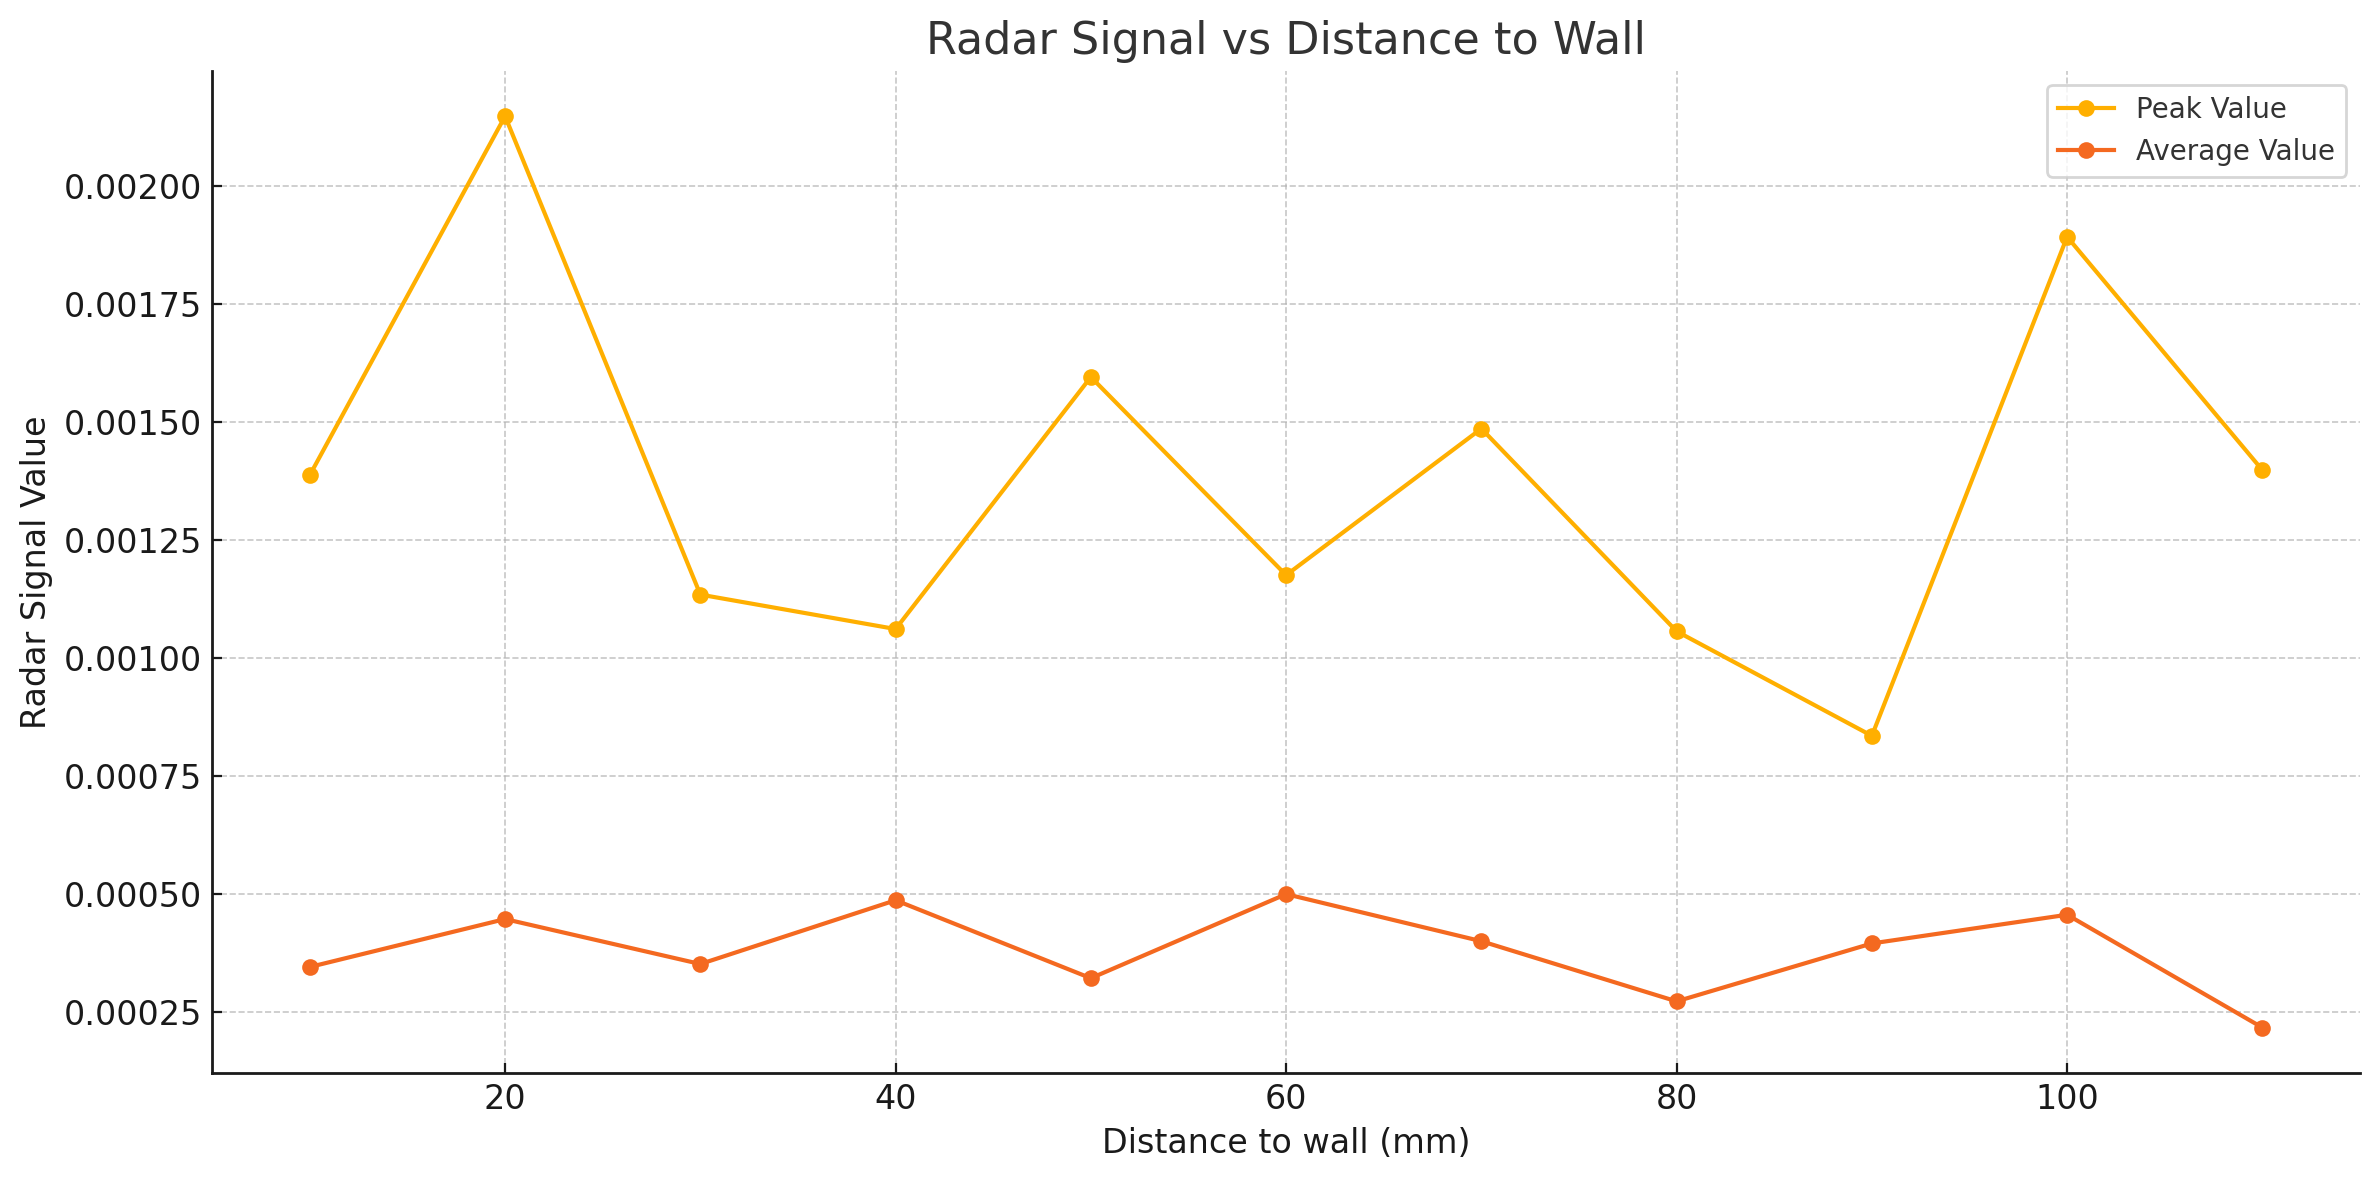
\includegraphics[width=\linewidth]{Src/images/radar to wall dist.png}
        \subcaption{Radar to Wall Distance}
        \label{fig:radar-wall}
    \end{minipage}
    \caption{Corridor layout and corresponding radar distance measurement.}
    \label{fig:corridor-radar-combo}
\end{figure}

The results indicate that as the radar approaches one of the walls, the signal amplitude increases because the main lobe of the beam pattern directly illuminates the wall at $0^{\circ}$. However, at distances less than 200 mm, the data about the wall become invalid due to strong near-field reflections and limitations in the radar’s resolution caused by its wide beam pattern. This leads to signal distortion, as reflections from the wall merge with noise or other parasitic reflections.

When the radar moves to the center of the corridor (approximately 0.6 m from both walls), the signal amplitude increases again. This occurs due to the simultaneous reception of reflections from both walls, which fall within the radar’s wide beam pattern. These reflections interfere, and their amplitudes add up, increasing the peak signal value. However, such interference creates ambiguities in data interpretation, as the radar cannot clearly distinguish reflections from the two walls.

If the radar is positioned strictly parallel to the wall, reflections from it can be minimized, as the main lobe of the beam pattern does not directly illuminate the wall, and most of the energy is radiated along the corridor. In this case, reflections from the side walls are significantly reduced, lowering the level of parasitic signals.




\begin{figure}[H]
    \centering
    \begin{minipage}[b]{0.8\linewidth}
        \centering
        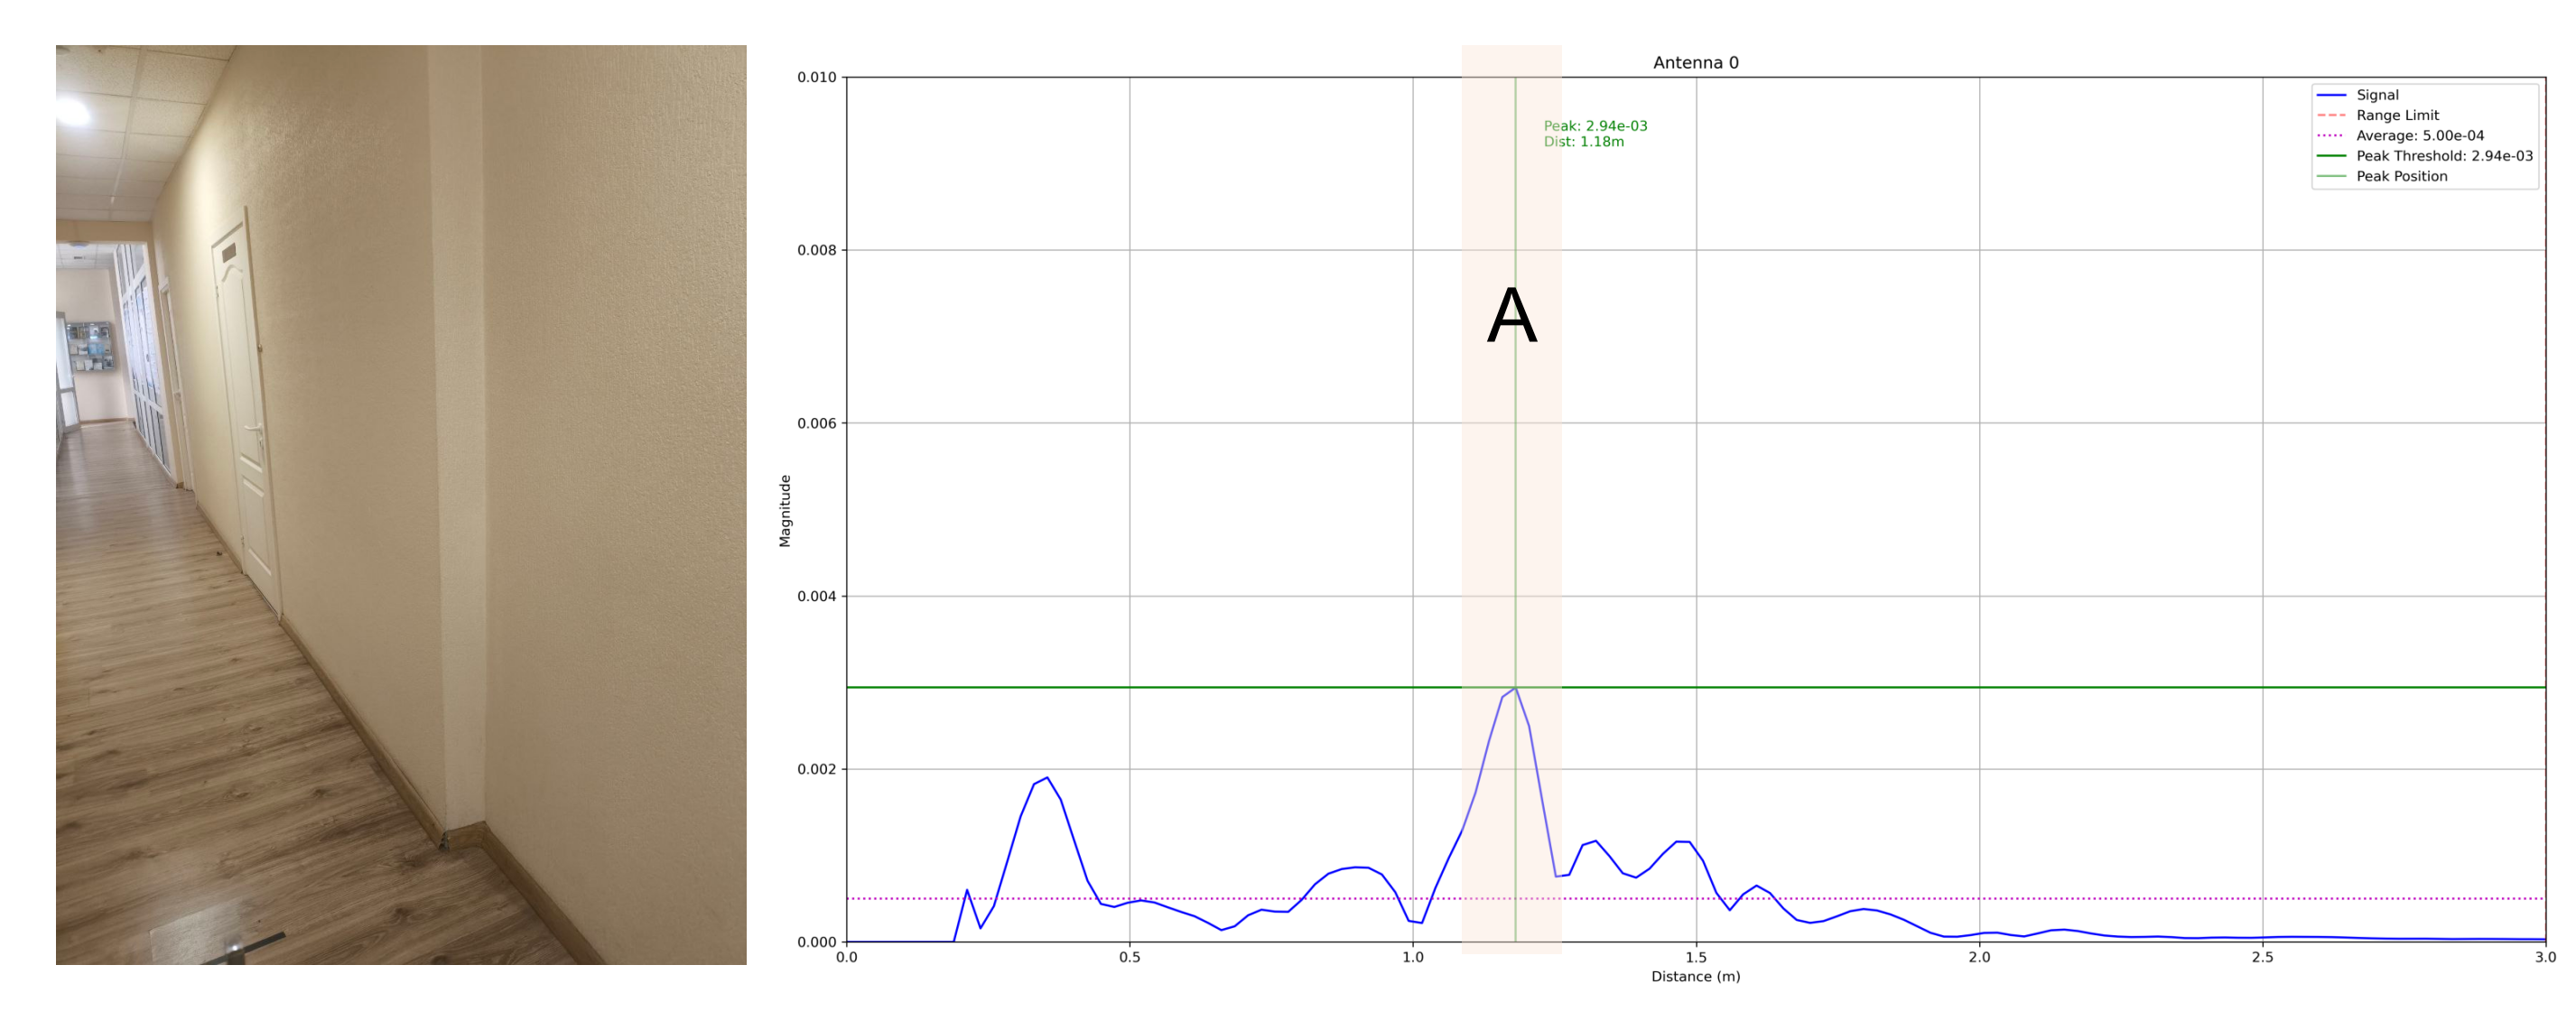
\includegraphics[width=\linewidth]{Src/images/coridora.png}
        \subcaption{First corner view}
        \label{fig:coridor-a}
    \end{minipage}
    \hfill
    \begin{minipage}[b]{0.8\linewidth}
        \centering
        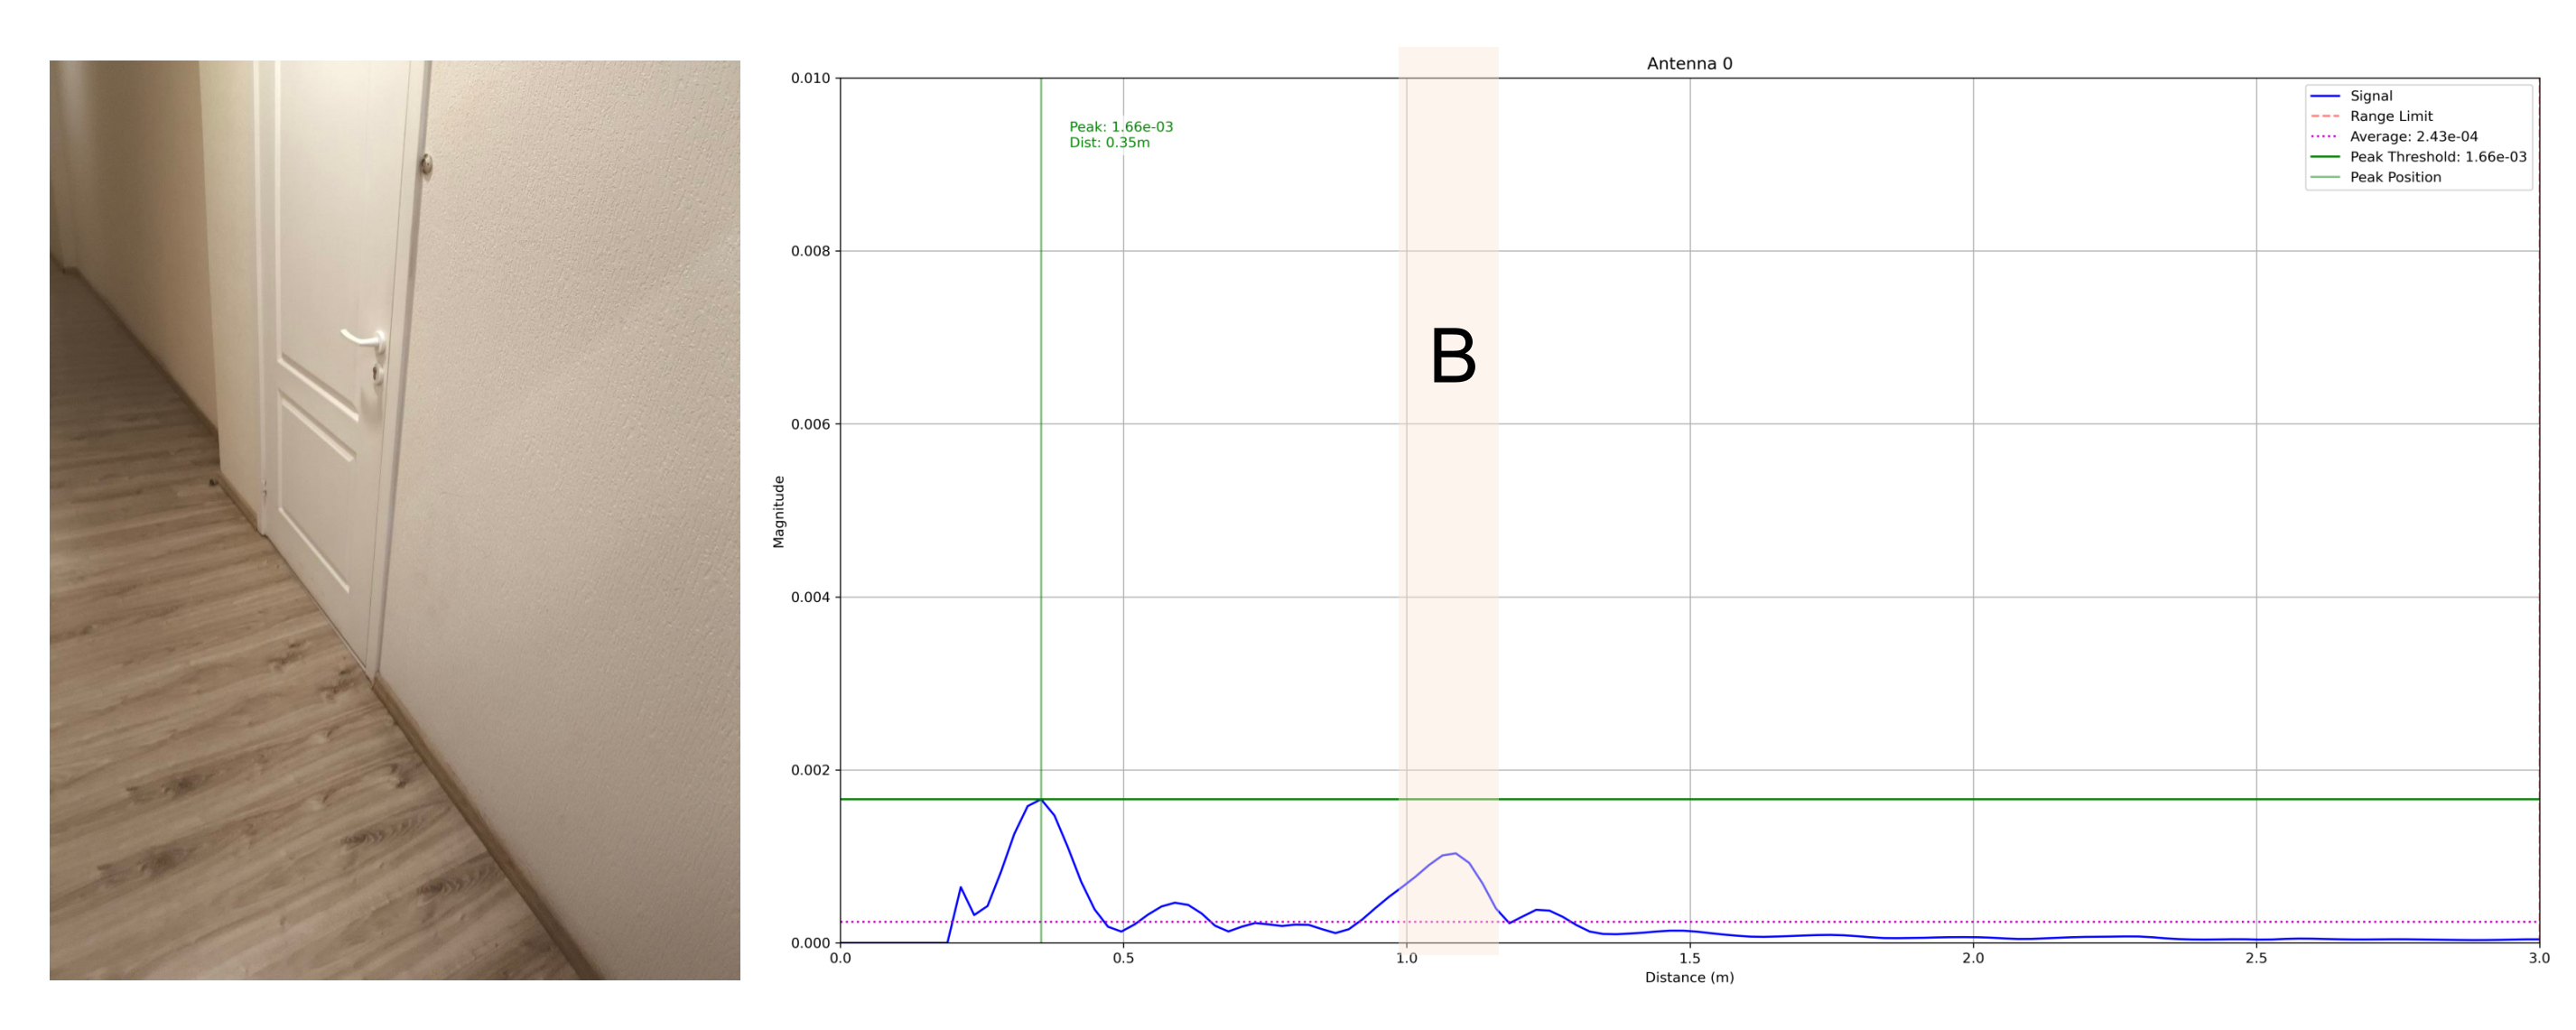
\includegraphics[width=\linewidth]{Src/images/coridorb.png}
        \subcaption{Second corner view}
        \label{fig:coridor-b}
    \end{minipage}
    \caption{Comparison of two corridor corners}
    \label{fig:corridor-comparison}
\end{figure}

Thus, in narrow corridors, object detection is limited not so much by signal strength but by ambiguities caused by multiple reflections and the radar’s wide beam pattern. For robotics applications, this implies the need to adapt signal processing algorithms to account for reflection interference and ensure accurate distance determination to walls.

During the testing of the radar, it was found that reflections are formed not only from the main objects, but also from the structural elements of the corridor, such as corners, edges and protruding structures. In Figure \ref{fig:corridor-comparison}, case \ref{fig:coridor-b}, it is shown that the radar captures the reflection from the door edge, highlighted in zone a, due to its geometry and material, amplifying the reflected signal. In the case of a larger protrusion, shown in the case of  \ref{fig:coridor-b}, in Figure \ref{fig:corridor-comparison}, the reflection intensity is noticeably higher due to the larger area of the reflecting surface and its shape, which contributes to signal amplification

\paragraph{Human Detection at Different Distances and Radar Heights}  
This experiment aimed to determine how the presence of a person influences radar output data depending on the radar’s height above the floor. The person was positioned at distances of 1 meter and 2 meters from the antenna. The graph in Figure \ref{fig:floor-human} illustrates the reflected signal’s peak value as a function of radar height, ranging from 0 to 1000 mm.  

As can be seen from Figure \ref{fig:floor-human}, the reflected signal from a person at a distance of 2 meters is more than twice as weak compared to the signal at a distance of 1 meter. This is due to lower propagation losses over the shorter distance. At a distance of 1 meter, the peak signal values are higher; however, they are highly modulated due to the person's natural micro-movements of limbs, which cause amplitude fluctuations.
\begin{figure}[H]
        \centering
    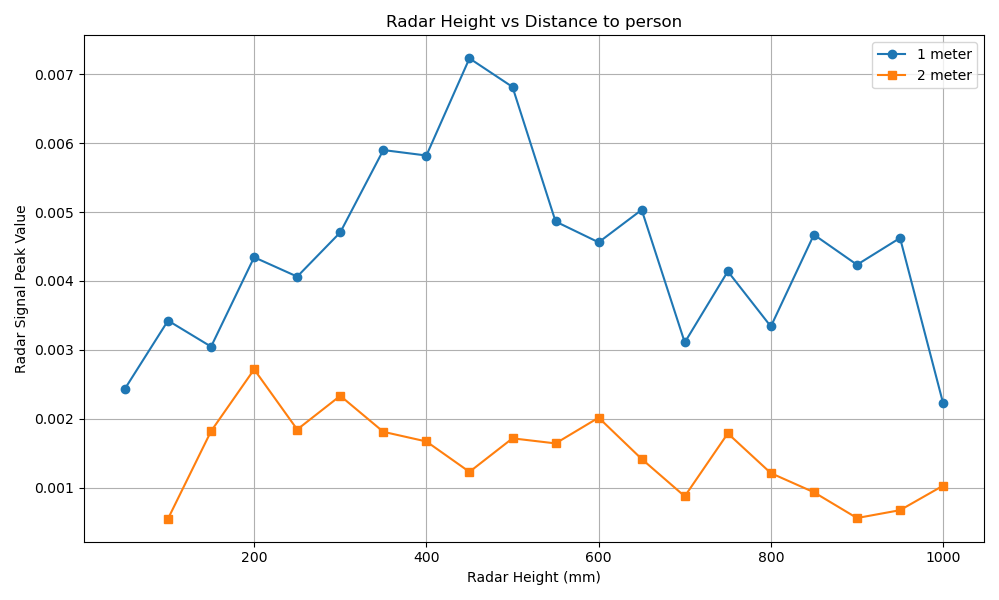
\includegraphics[width=0.8\linewidth]{Src/images/radar flor men.png}
    \caption{Reflections from a person at 1 m and 2 m for different radar heights }
    \label{fig:floor-human}
\end{figure}

The strongest and most stable reflections, providing the best signal-to-noise ratio, are observed when the radar height is approximately from 400 to 600 mm (or about 0.5 meters above the radar). When the radar is positioned close to the floor (at knee level), the received signal is affected by both the floor itself and the person's legs. Legs can be represented as two cylindrical objects, from which the reflection scatters more strongly than from the torso, which can lead to the signal level dropping below the detection threshold. With an increase in distance to 2 meters, the received signals become less stable, and their values can vary significantly over time, which complicates the task of reliably detecting a person. At the same time, raising arms or changing posture, which increases the reflective area (radar cross-section) towards the radar, can lead to a more stable signal peak.


\begin{figure}
    \centering
    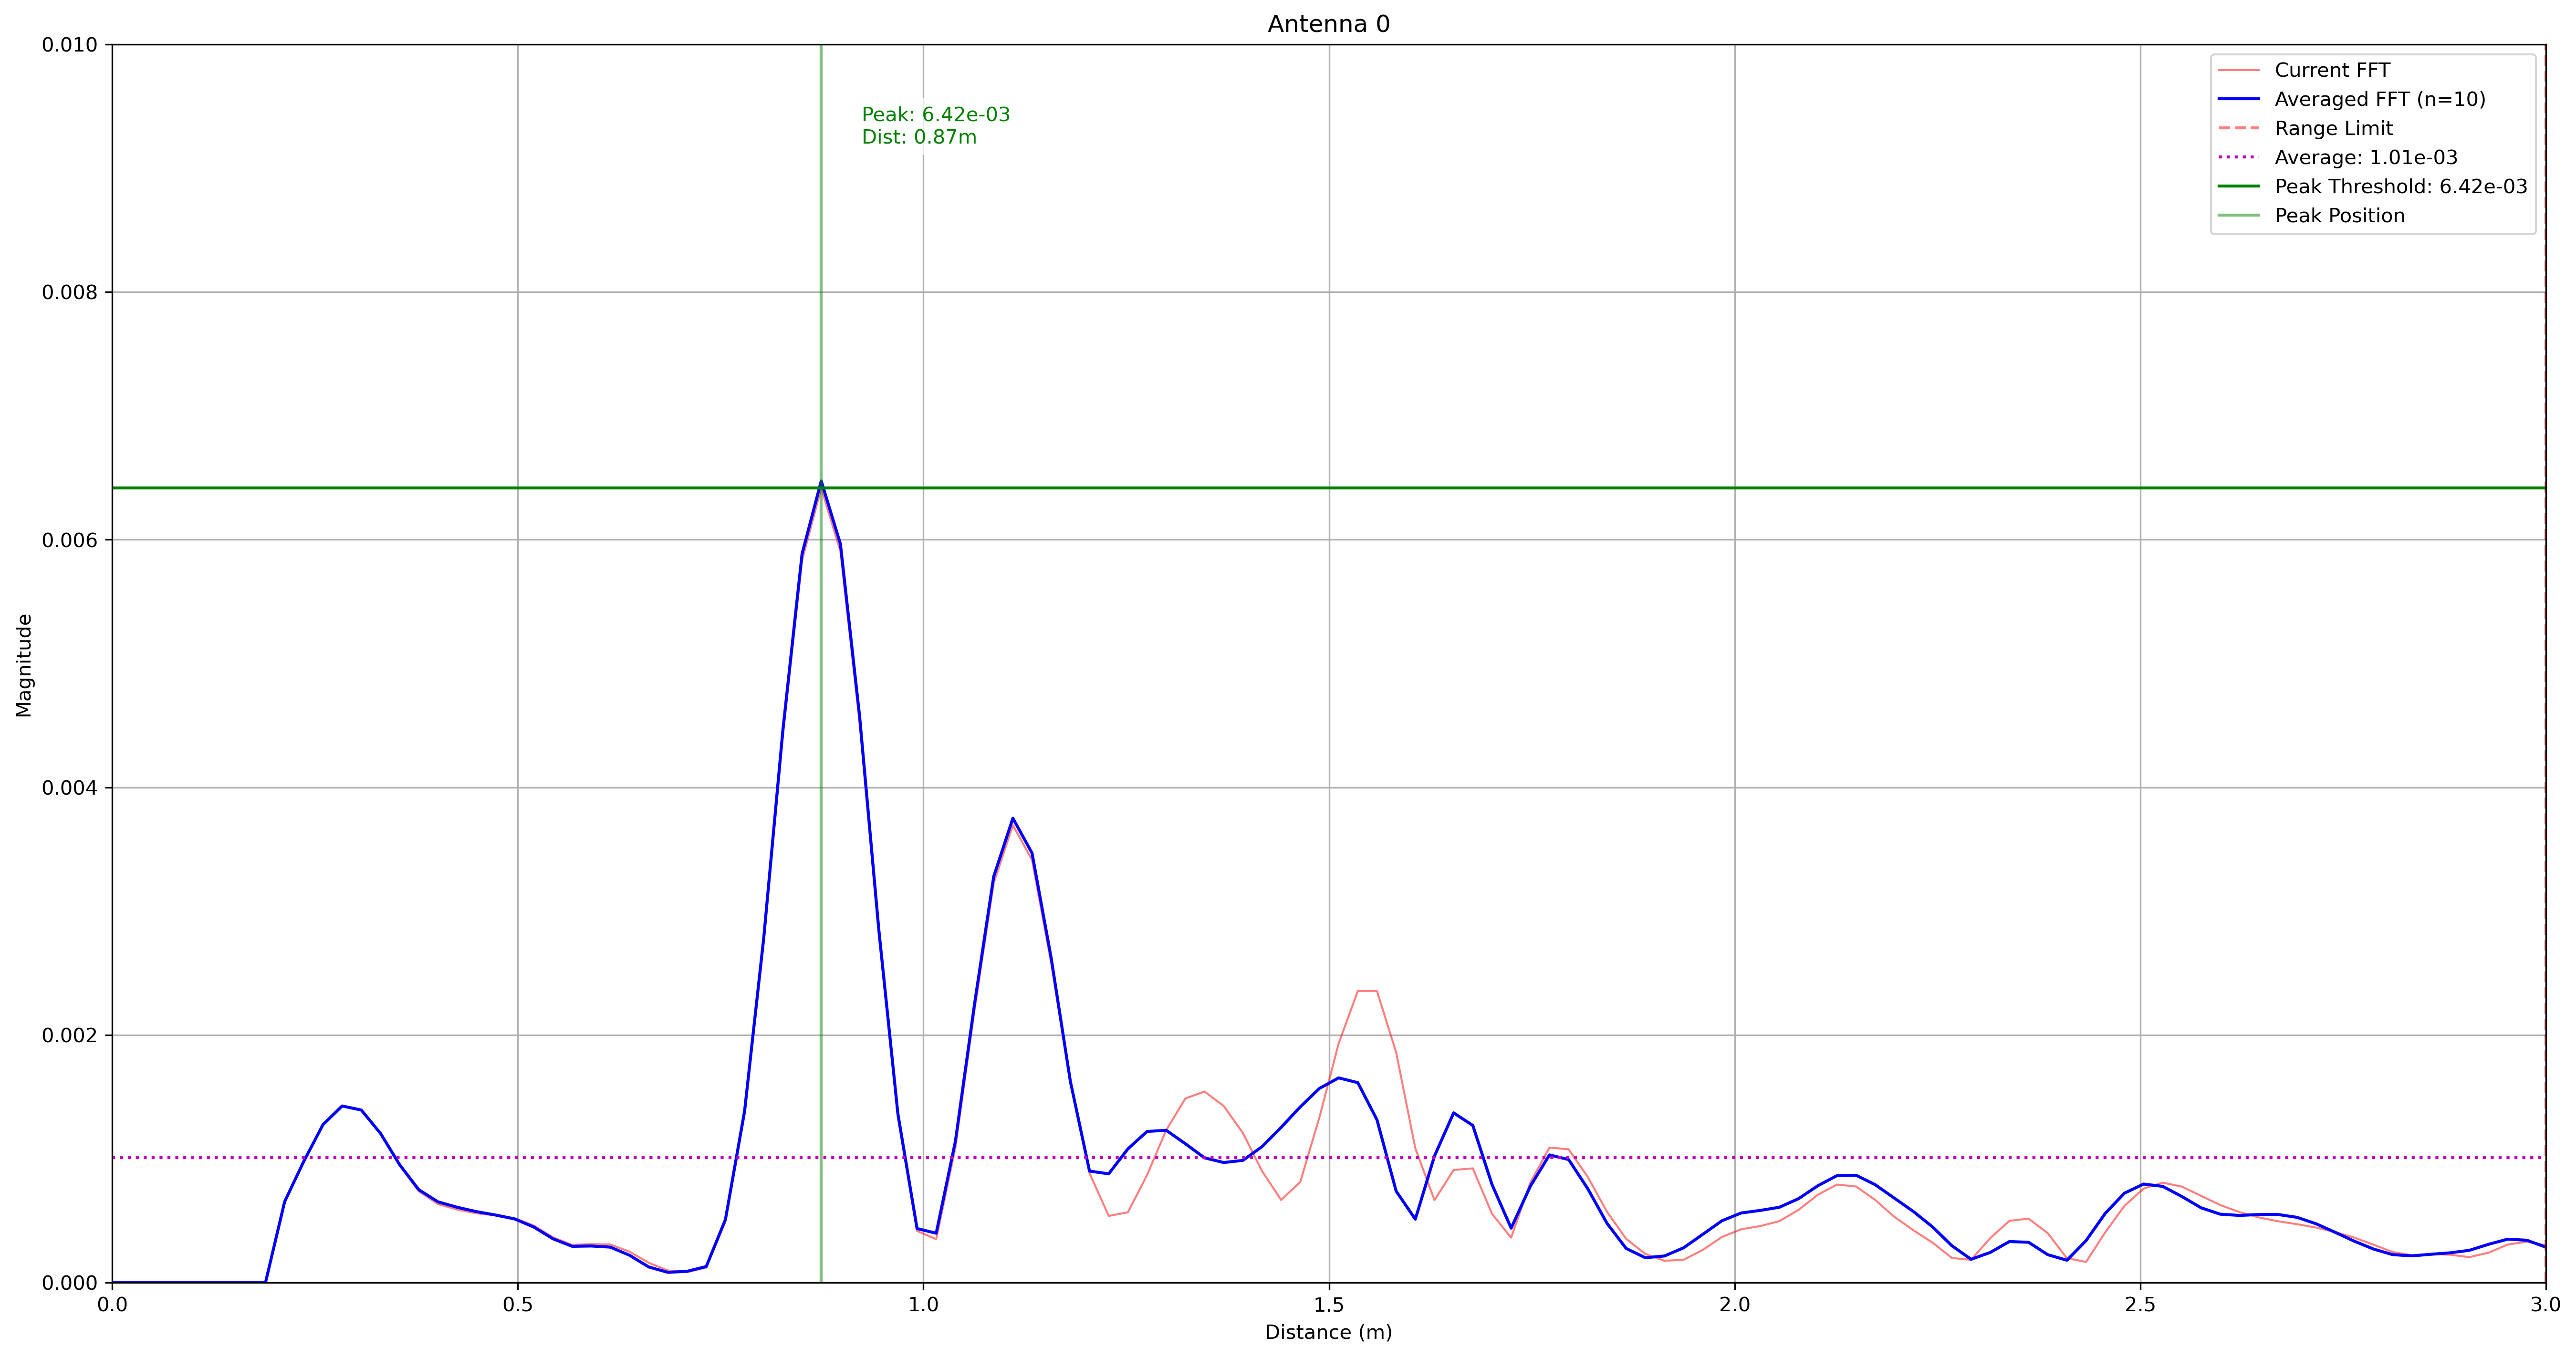
\includegraphics[width=0.75\linewidth]{Src/images/radar_plot.png}
    \caption{Reflected radar signal magnitude highlighting the effect of temporal accumulation in improving signal clarity.}

    \label{fig:signal-clarity}
\end{figure}


When the radar is placed at the height of the leg, the reflected signal spectrum exhibits a stable `pedestal' in the range of 0.8–1.2\,m. This component arises from the combined scattering from both shins and mirror reflections from the floor. Due to the relatively static geometry of the legs, the instantaneous amplitude of this component varies no more than ±10–15\% from its average value and often approaches the noise level, especially at a distance of 2\,m.

To reliably detect this weak but persistent reflection, sliding frame accumulation over a window of \(N\) frames is used: each new spectrum is added to the sum of the previous \(N-1\) values, then the result is normalized by \(N\). Under such integration, the standard deviation of the noise decreases as \(1/\sqrt{N}\); for \(N = 10\), it is reduced by a factor of approximately 3.2.

A window of 10 frames provides a practical trade-off: it reduces noise, and introduces a detection delay of no more than 0.5–1\,s at a frame rate of 10\,Hz.

As shown in Figure \ref{fig:signal-clarity}, the blue curve illustrates the effect of 10-frame accumulation, clearly highlighting the leg-level reflection pedestal, while the red curve represents a single FFT frame.\citep{Skolnik2001} 

As a result, the optimal configuration to reliably detect human presence within 1–2\,m includes placing the radar at a height of \(0.45 \pm 0.1\,\mathrm{m}\), using accumulation over 10–12 frames, and applying a dynamic detection threshold set at least \(5\sigma\) above the estimated noise level. For targets at 2\,m, increasing the integration time to 16–20 frames ensures a detection probability of at least 0.9. .


\paragraph{Influence of object rotation}
% Describing mmWave properties
Millimeter waves, also known as mmWave, operate in the frequency range of 24 to 300 gigahertz, which corresponds to wavelengths of approximately 1 to 12.5 millimeters.

Due to their short wavelength, mmWave exhibit characteristics similar to those of light waves. They tend to travel in a straight line, and their behavior is well described by the principles of geometric optics, such as the law of reflection (the angle of incidence is equal to the angle of reflection). This means that mmWave behaves like rays, particularly in environments where the dimensions of objects (such as walls and furniture) are significantly larger than the wavelength.\citep{rappaport2002wireless,li2022ground}.

\begin{figure}[H]
    \centering
    \begin{minipage}[b]{0.95\linewidth}
        \centering
            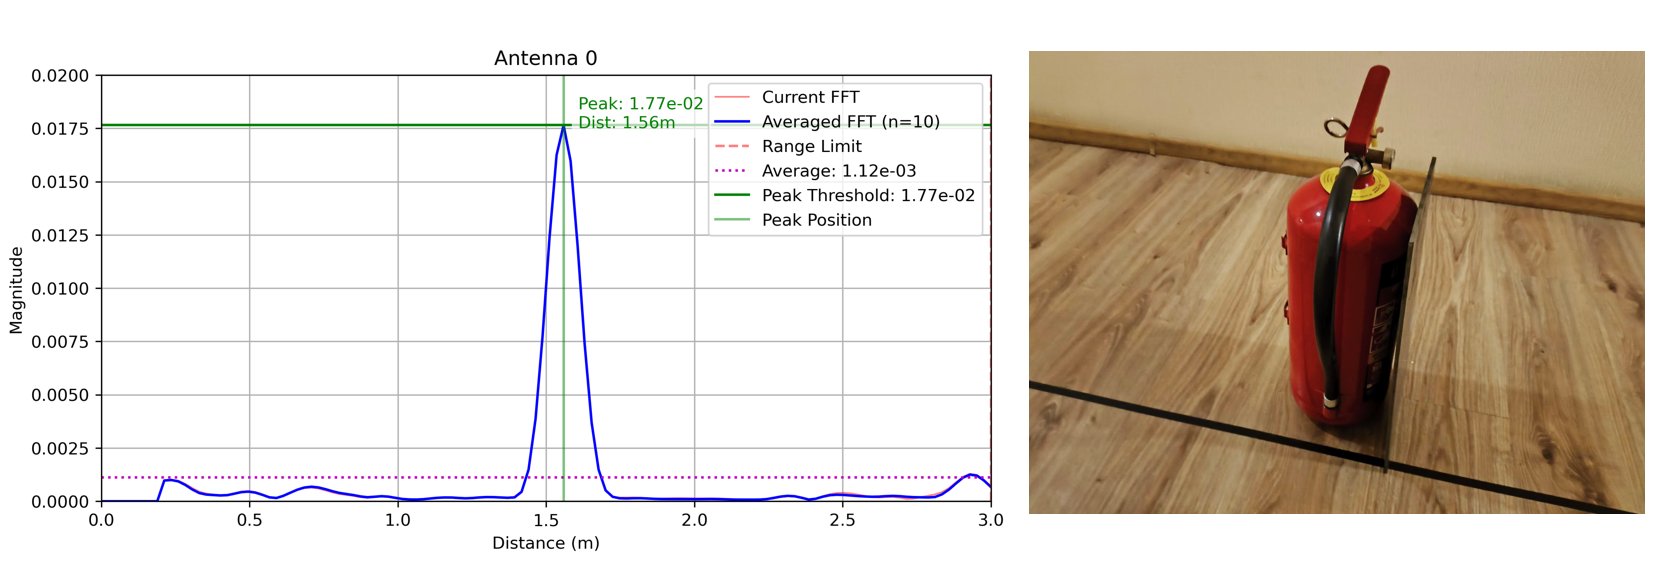
\includegraphics[width=1\linewidth]{Src//images/ognfft.png}

        \subcaption{Plate perpendicular to the plane}
        \label{fig:object-position-a}
    \end{minipage}
    \hfill
    \begin{minipage}[b]{0.95\linewidth}
        \centering
            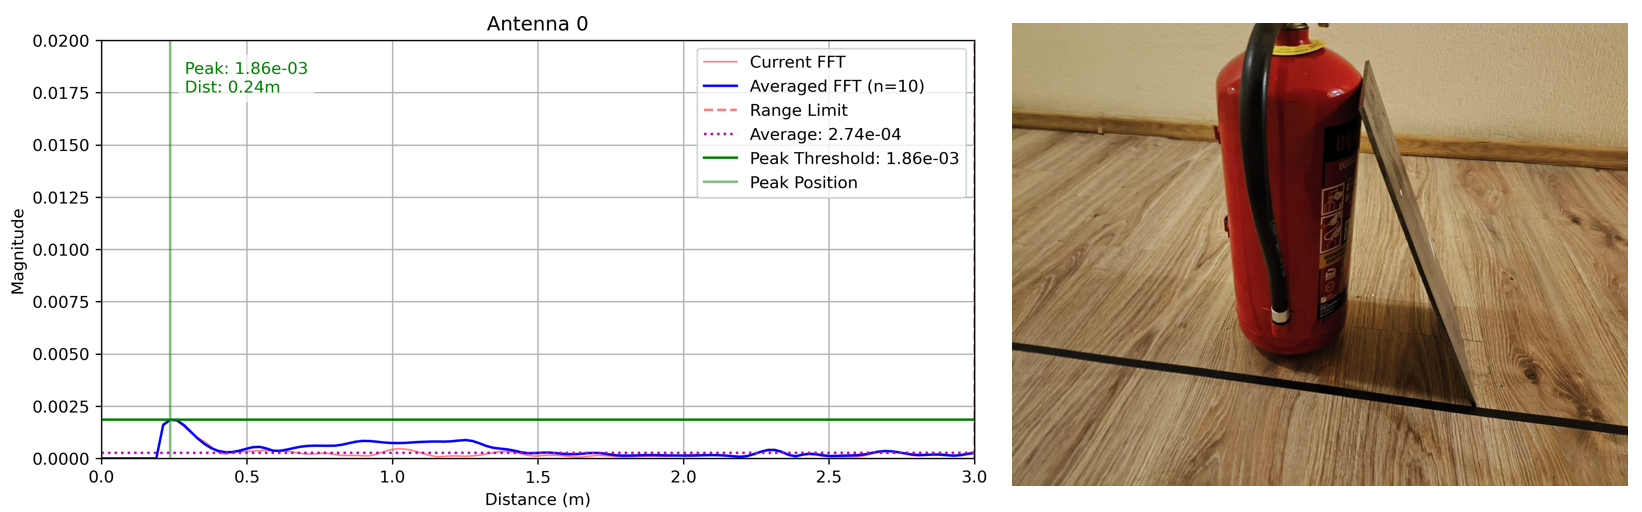
\includegraphics[width=1\linewidth]{Src//images/ognfft2.png}

        \subcaption{The plate 45 \degree relative to the radar.}
        \label{fig:object-position-b}
    \end{minipage}
    \caption{Metal plate in form of a reflector.}
    \label{fig:object-position-comparison}
\end{figure}

Thus, as shown in Figure~\ref{fig:object-position-comparison}, the orientation of an object relative to the radar's radiation axis critically affects the level of the received reflected signal.



\begin{figure}[H]
    \centering
    \begin{minipage}[b]{0.3\linewidth}
        \centering
        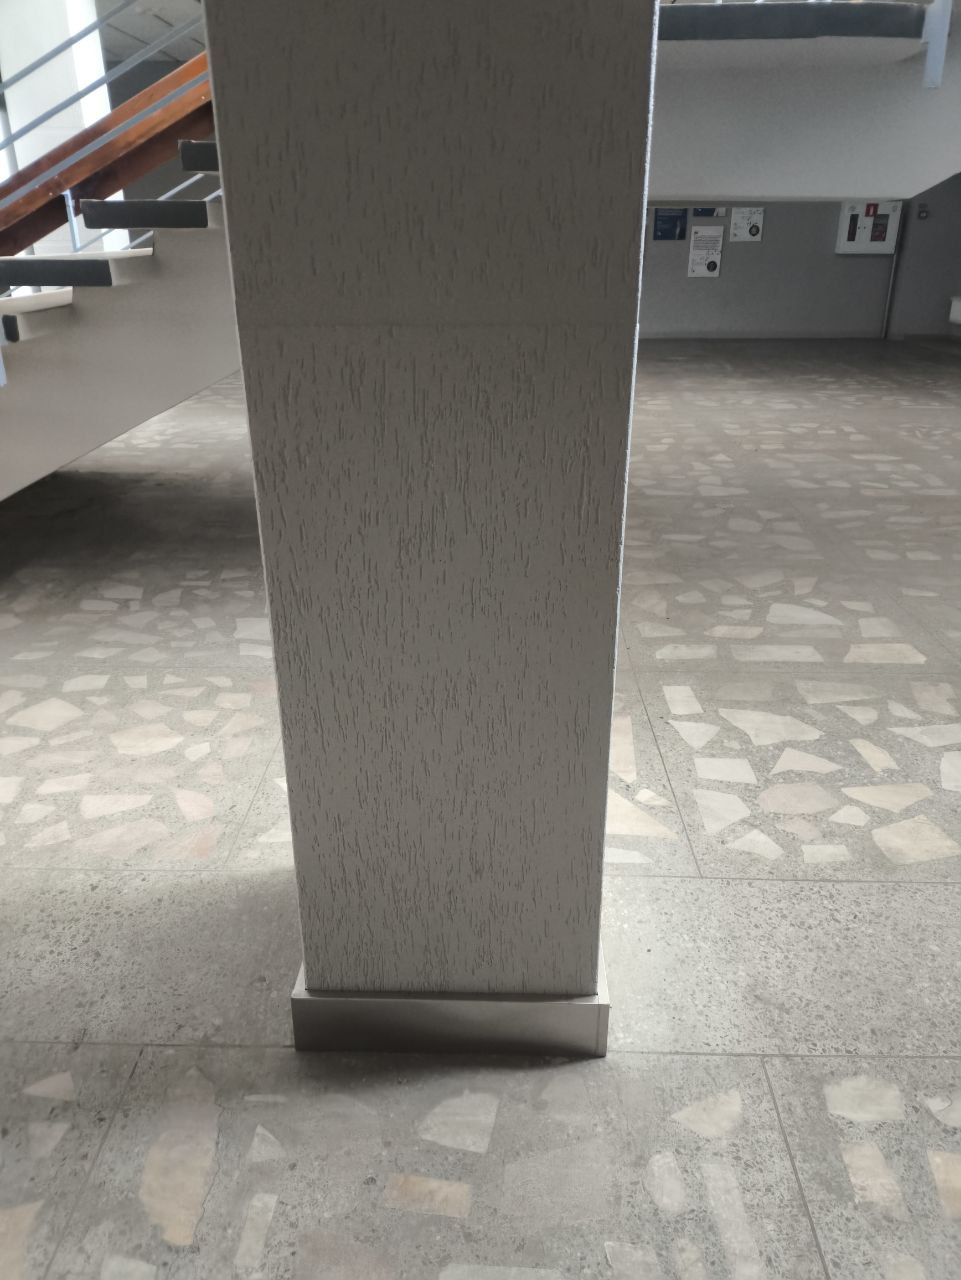
\includegraphics[width=\linewidth]{Src/images/photo_5906680020825392807_y.jpg}
        \subcaption{Radar located perpendicular}
        \label{fig:rotation-a}
    \end{minipage}
    \hfill
    \begin{minipage}[b]{0.3\linewidth}
        \centering
        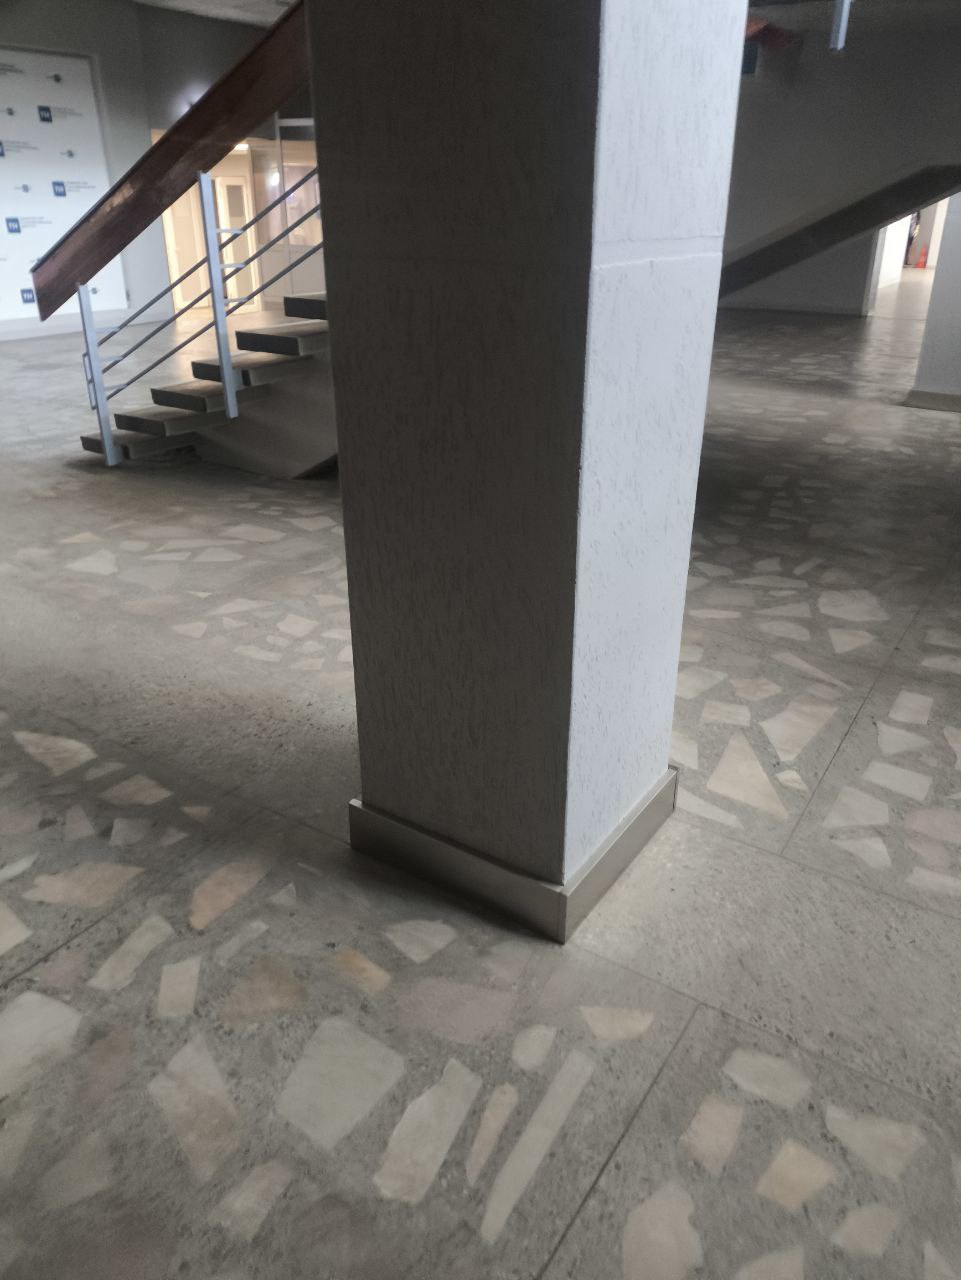
\includegraphics[width=\linewidth]{Src/images/photo_5906680020825392808_y.jpg}
        \subcaption{Radar located at 45 \degree}
        \label{fig:rotation-b}
    \end{minipage}
    \hfill
    \begin{minipage}[b]{0.3\linewidth}
        \centering
        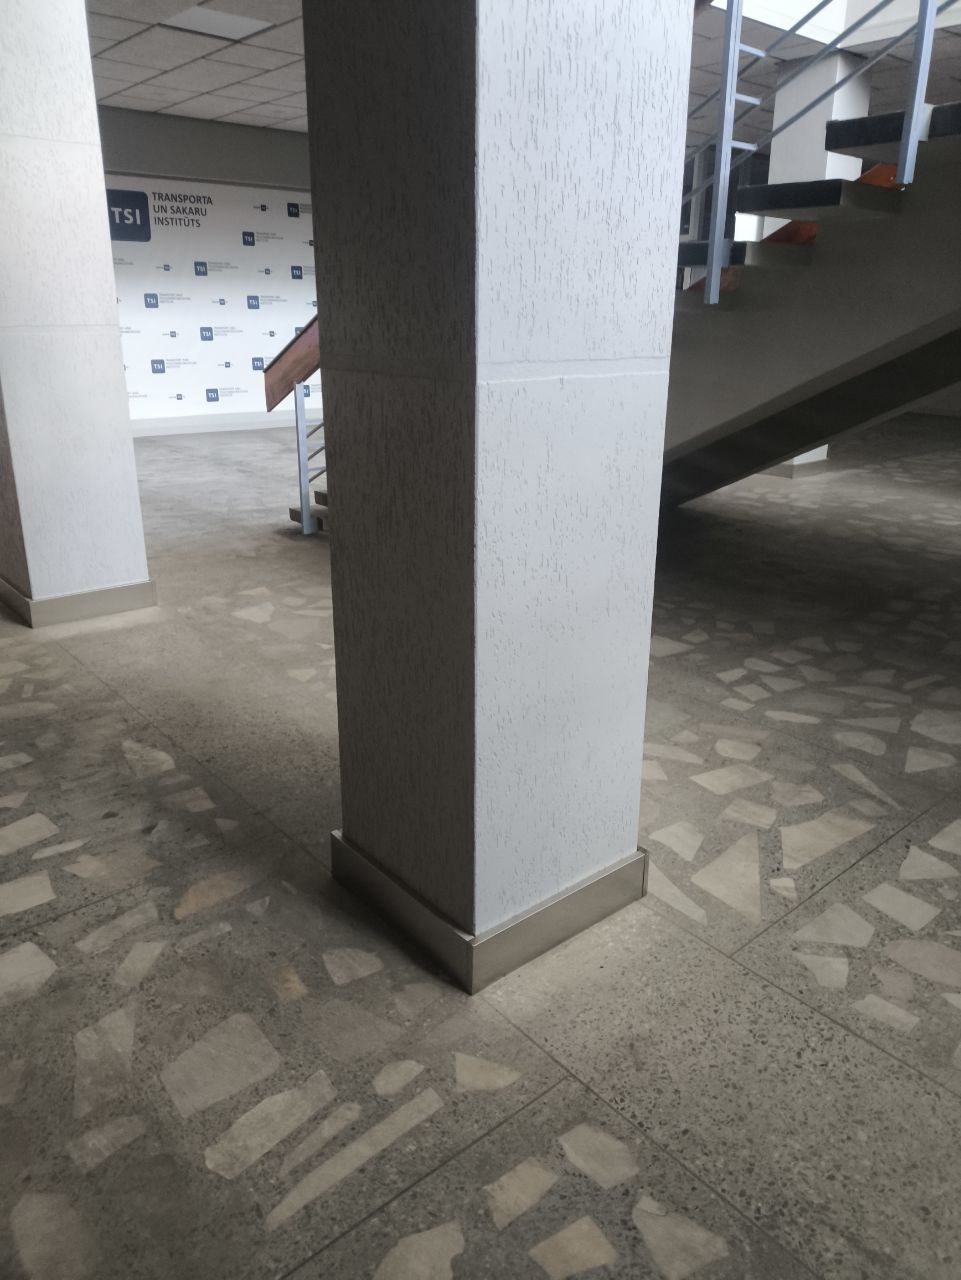
\includegraphics[width=\linewidth]{Src/images/photo_5906680020825392809_y.jpg}
        \subcaption{Radar located at 75 \degree}
        \label{fig:rotation-c}
    \end{minipage}
    \caption{Reflection from the column.}
    \label{fig:object-rotation}
\end{figure}
 When the metal plate is positioned perpendicular to the beam (Figure~\ref{fig:object-position-a}), the reflection is directed back to the receiver, and the signal is recorded with high amplitude. However, when tilted at an angle of 45° (Figure~\ref{fig:object-position-b}), a significant portion of the energy is deflected to the side, and the reflection weakens.
 
A similar situation is observed during interaction with indoor objects, such as columns or wall corner protrusions. Figure~\ref{fig:object-rotation} presents real examples of reflections from a column at various angles of radar installation. When the radar is aimed strictly perpendicular to the object (Figure~\ref{fig:rotation-a}), the reflection is clearly recorded. However, when tilted 45 \degree (Figure~\ref{fig:rotation-b}), the signal becomes less pronounced and at an angle of 75 \degree (Figure~\ref{fig:rotation-c}), the reflected energy practically does not return to the receiving antenna.

Consequently, objects with high reflectivity, such as metal structures or the sharp corners of columns, can completely "disappear" from the radar map when oriented at an angle greater than 45 \degree. This poses a particular danger for the navigation of mobile robots or detection systems, as such elements cannot be reliably detected under any conditions. This is especially critical in complex indoor environments where the presence of such "invisible" obstacles can lead to failures in environmental perception.

\subsubsection{Dielectric Box Thickness Estimation}\label{sec:box-thickness}

\textbf{Purpose.} Verify the feasibility of noncontact thickness measurement for the two orthogonal sides of a multilayer cardboard box (dielectric material; Section 3.5.1)  
This method can also be used to detect and classify dielectric objects with internal layers or stacked structures: If the spacing between the two dominant reflection peaks remains constant across multiple radar positions but their absolute range shifts, this indicates internal propagation and confirms the dielectric nature of the object. Alternatively, such behavior may suggest that an additional object is located behind the primary target.

\textbf{Test object.} Multilayer cardboard box Figure \ref{fig:box}.  
Two inner spacings are of interest:  
shorter side — \(d_{\text{true,short}} \approx 26\,\text{cm}\);  
longer side — \(d_{\text{true,long}}  \approx 59\,\text{cm}\).
\textbf{Method.}  
For each side the following steps are executed:
\begin{enumerate}
    \item Place the FMCW radar at two fixed ranges from the illuminated wall:
          \begin{itemize}
              \item \emph{Near position}: \(R_{1} \approx 0.5\,\text{m}\);
          \end{itemize}
    \item Transmit a linearly frequency-modulated waveform; the wave penetrates the front wall and reflects from the rear wall.
    \item Apply a 1-D Fast Fourier Transform (FFT) to obtain the range profile.
    \item Detect two dominant peaks: \(\mathrm{Peak}_{\text{front}}\) (front wall) and \(\mathrm{Peak}_{\text{back}}\) (rear wall).
    \item Compute the spacing \(\Delta R = \lvert R_{\text{back}} - R_{\text{front}}\rvert\) and estimate thickness
          $
              d_{\text{est}} = \frac{c\,\Delta R}{2n},
          $
          where \(c\) is the speed of light and \(n\) is the effective refractive index of cardboard.
    \item Repeat the measurement \(N\) times for each range; obtain the mean \(\overline{d}_{\text{est}}\) and standard deviation \(\sigma\) separately for the short and long sides.
\end{enumerate}

\begin{figure}[H]
    \centering
    \begin{minipage}[t]{0.6\linewidth}
        \centering
        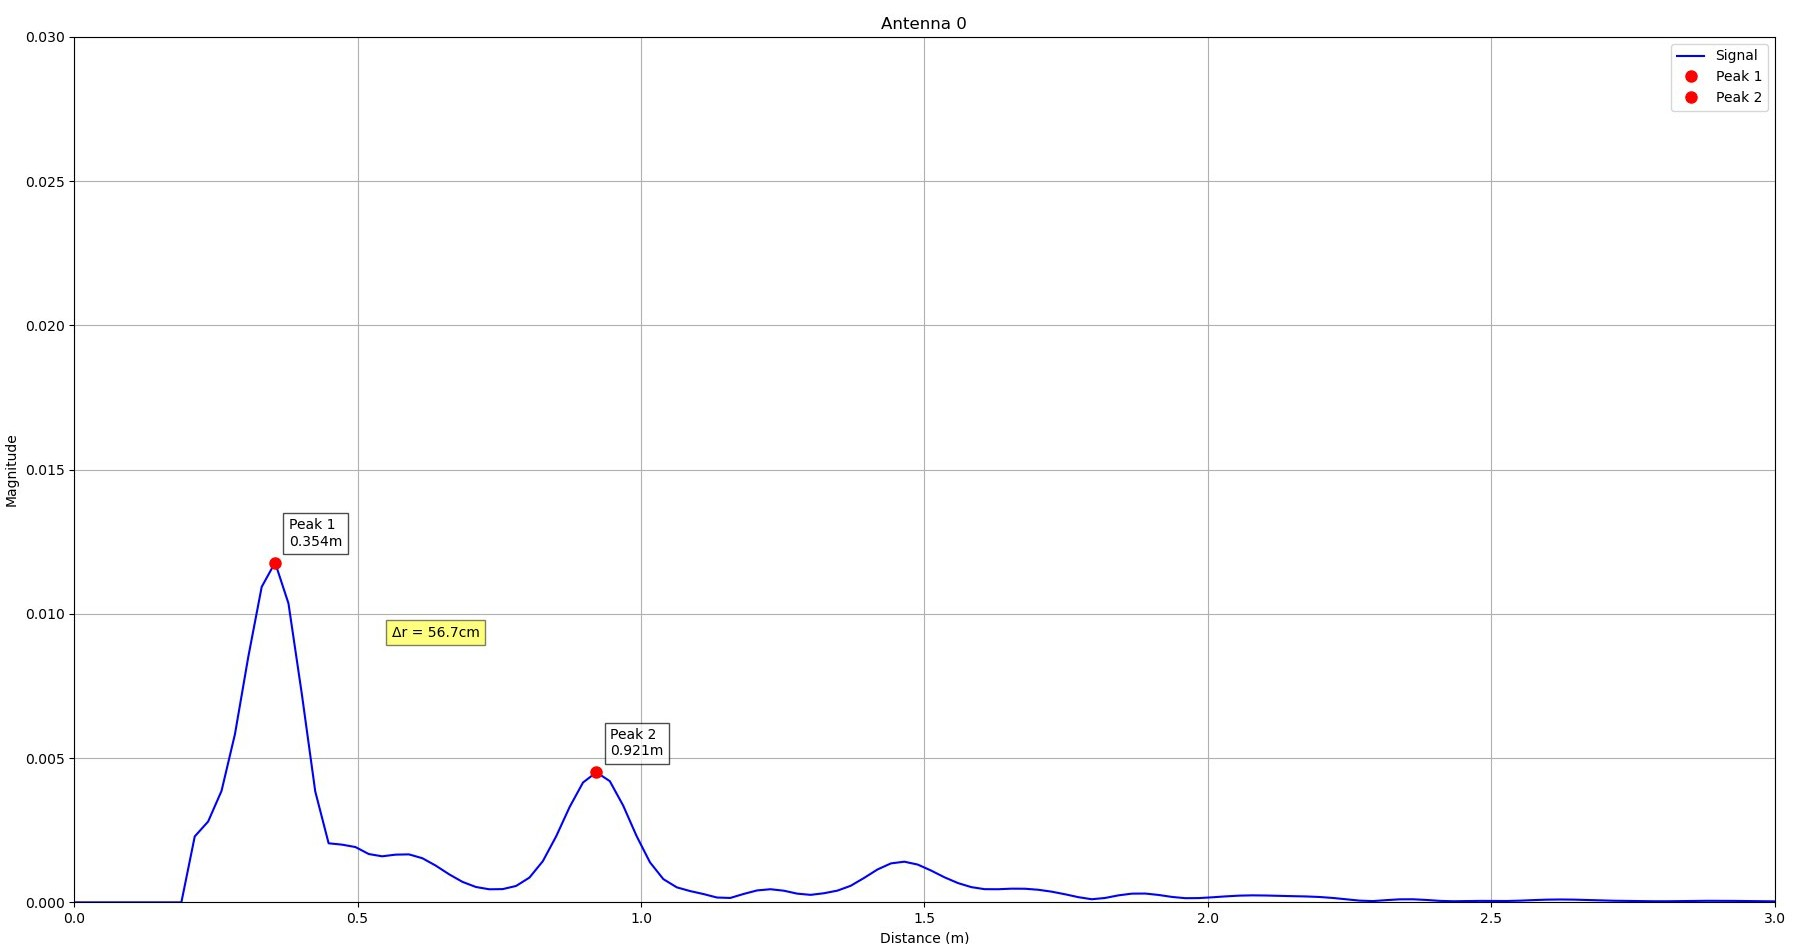
\includegraphics[width=\linewidth]{Src/images/mox_measurmentL.jpg}
        \caption{Range profile for the \textbf{longer} side.  
                 Front and rear peaks at \(0.354\) m and \(0.921\) m indicate a wall spacing of \(56.7\) cm.}
        \label{fig:box-long-profile}
    \end{minipage}\hfill
    \begin{minipage}[t]{0.6\linewidth}
        \centering
        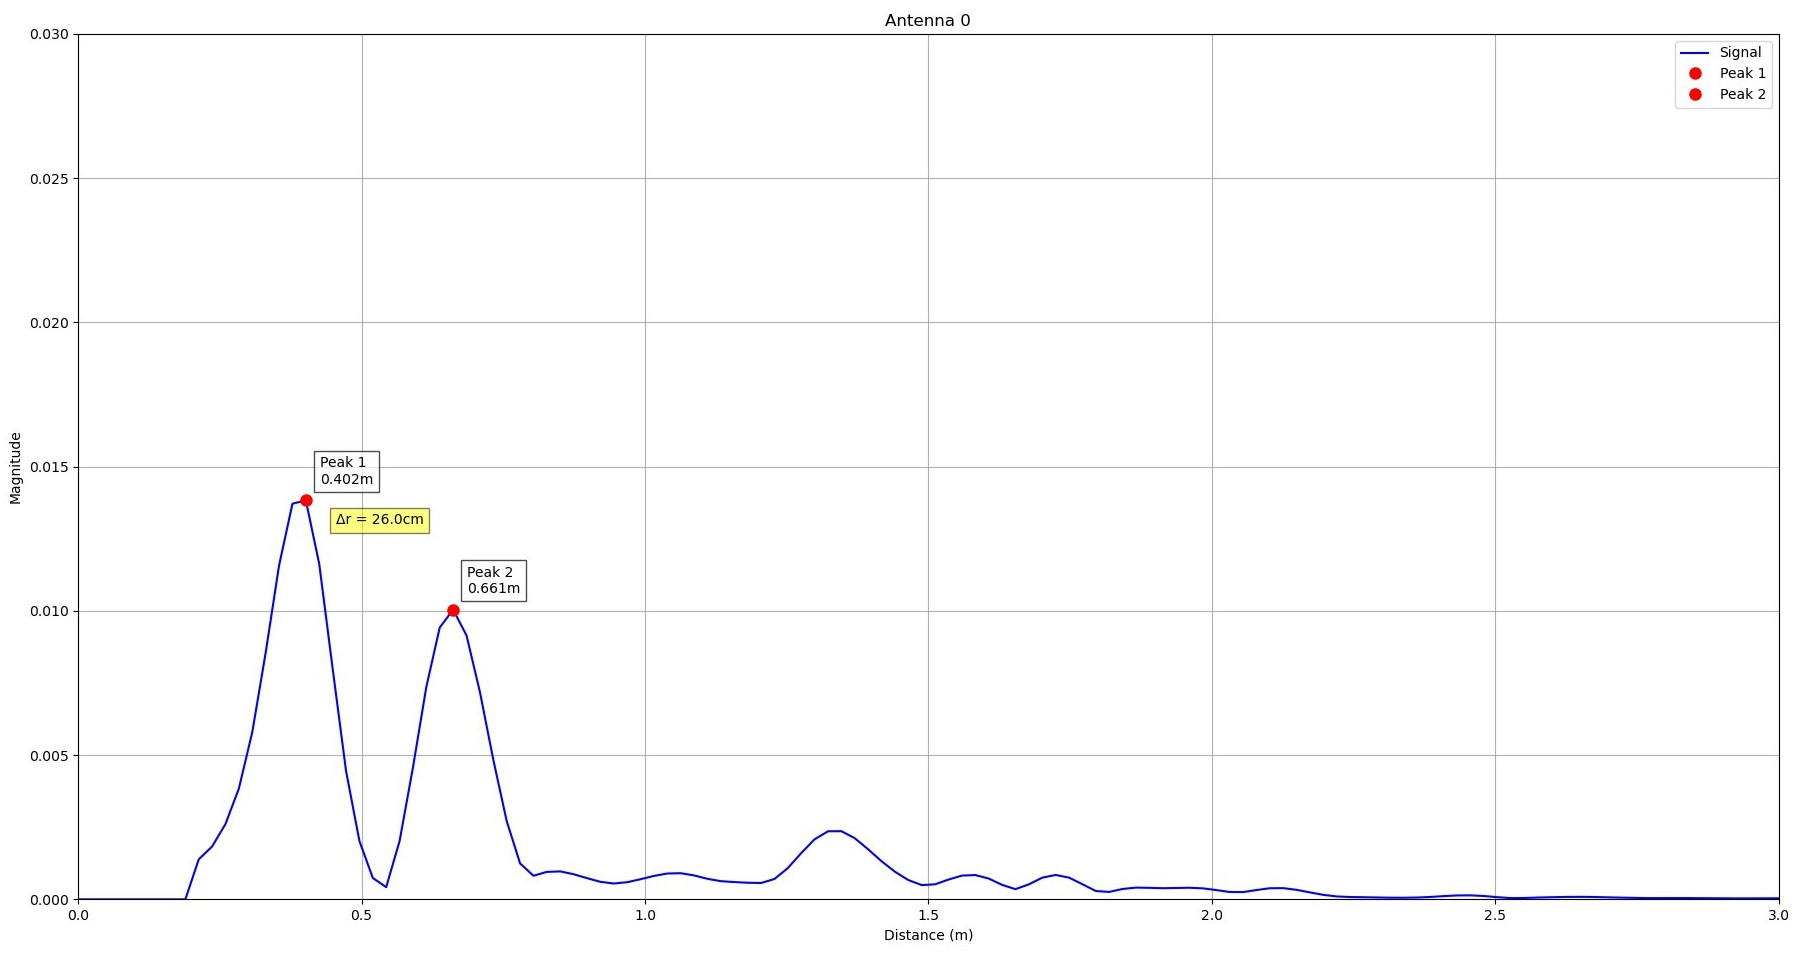
\includegraphics[width=\linewidth]{Src/chapters/mox_measurmentS.jpg}
        \caption{Range profile for the \textbf{shorter} side.  
                 Peaks at \(0.402\) m and \(0.661\) m yield the expected \(26.0\) cm spacing.}
        \label{fig:box-short-profile}
    \end{minipage}
\end{figure}

\paragraph{Result.}
Figures \ref{fig:box-long-profile}–\ref{fig:box-short-profile} present the resulting spectra.
For both sides the radar distinctly resolves the front and rear reflections; the highlighted spacing \(\Delta R\) is the basis for thickness estimation.

\begin{itemize}
    \item \textbf{Longer side (Figure\,\ref{fig:box-long-profile}).}  
          \(R_{\text{front}} = 0.354\,\text{m}\), \(R_{\text{back}} = 0.921\,\text{m}\),   
          \(\Delta R = 0.567\,\text{m}\) \(\Rightarrow\)
          \(d_{\text{long,est}} = 56.7\,\text{cm}\).  
          \textit{Error:} \(\varepsilon_{\text{long}} = d_{\text{long,est}} - d_{\text{true,long}}
          = -2.3\,\text{cm}\;(-3.9\%)\).

    \item \textbf{Shorter side (Figure\,\ref{fig:box-short-profile}).}  
          \(R_{\text{front}} = 0.402\,\text{m}\), \(R_{\text{back}} = 0.661\,\text{m}\),   
          \(\Delta R = 0.260\,\text{m}\) \(\Rightarrow\)
          \(d_{\text{short,est}} = 26.0\,\text{cm}\).  
          \textit{Error:} \(\varepsilon_{\text{short}} = d_{\text{short,est}} - d_{\text{true,short}}
          = 0.0\,\text{cm}\;(0.0\%)\).
\end{itemize}

Despite the accurate determination of thickness, it is important to note that the amplitude of the second (rear wall) reflection decreases as the internal spacing increases. This attenuation limits the maximum measurable thickness: based on the observed SNR, reliable detection becomes a challenge beyond approximately \(65\text{–}70\,\text{cm}\). Furthermore, as the entire object moves farther from the radar, both reflections experience overall signal weakening, further reducing the peak contrast and range resolution.

To ensure stable and precise measurements, especially at longer ranges, it is recommended to perform acquisition in static conditions. Motion-induced fluctuations or rapid changes in alignment lead to spectral smearing, making it difficult to isolate the rear-wall echo.


%------------------------------------------------------------
\subsubsection{Determination of Object Velocity}\label{sec:velocity_test}
%------------------------------------------------------------

\paragraph{Purpose.}
To verify the radar’s capability to estimate radial velocity via Doppler shift and to separate moving targets from static clutter.

\paragraph{Procedure.}
\begin{enumerate}
    \item Move a target (human, small robot, or pet) directly toward and away from the radar at controlled speeds.
    \item Collect multiple chirps per frame and apply a \textbf{2-D FFT}: 1-D over range, 2-D over slow-time (chirp index) to obtain a range–Doppler map.
    \item Extract the Doppler bin corresponding to maximum target energy and convert to velocity using
    $
        v = \frac{\lambda f_d}{2},
    $
    where $\lambda$ is the radar wavelength and $f_d$ is the Doppler frequency.
\end{enumerate}

\paragraph{Expected outcome.}
The radar should estimate radial velocities in the interval $\pm$1–2 m/s, while static objects remain near the zero-Doppler axis, enabling clear separation.

\paragraph{Environmental Noise Testing.}
Before conducting the main experiments, preliminary static measurements were performed under two contrasting conditions:  
(1) outdoors in an open area without reflective surfaces nearby, and  
(2) indoors in a workshop environment, surrounded by walls and metallic structures.

As shown in Figure \ref{fig:dopplere2}, scenario (1) demonstrates a uniform noise distribution across all ranges and Doppler bins, indicating minimal interference.  
In contrast, scenario (2) reveals a pronounced stationary clutter component along the zero-Doppler axis. This is attributed to strong multipath reflections caused by surrounding metallic equipment and nearby walls, which introduce unwanted static returns and degrade dynamic target separation.  
Such observations justify the need for high-pass Doppler filtering (MTI) in indoor experiments to suppress static clutter and separate moving targets.



\begin{figure}[H]
    \centering
    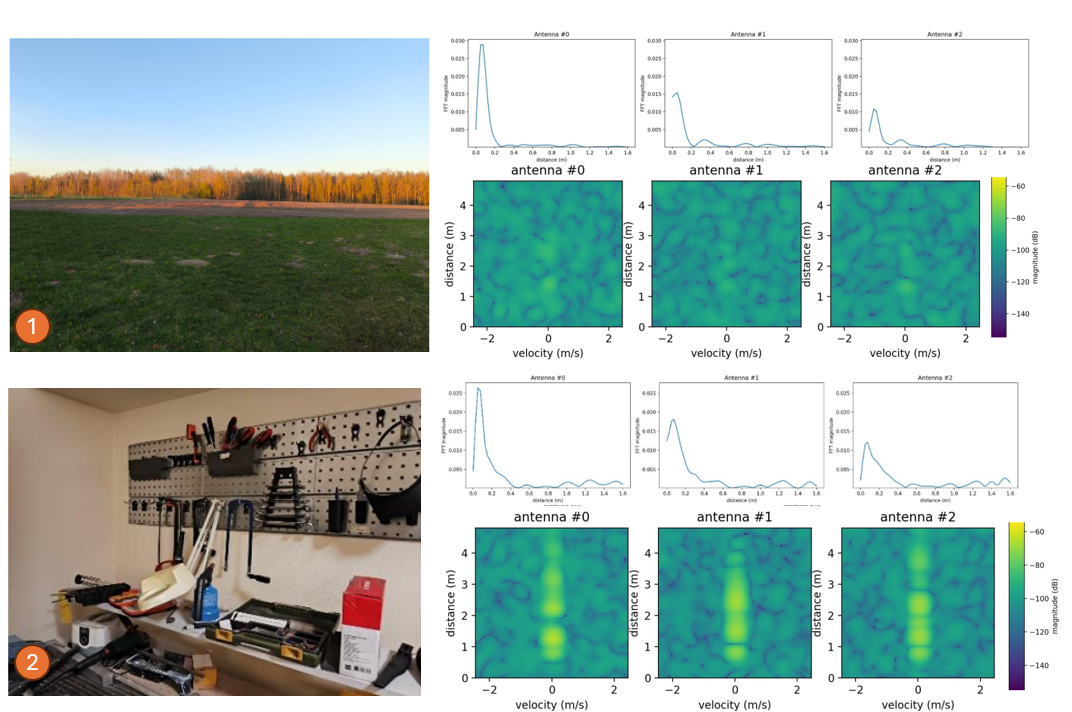
\includegraphics[width=\linewidth]{Src/images/doplere22.png}
    \caption{Static FFT and Doppler plot in open outdoor space(1) and workshop(2)indor}
    \label{fig:dopplere2}
\end{figure}


\paragraph{Pre-processing Chain.}
Prior to velocity and angle estimation, each data cube was passed through a three-stage pre-processing pipeline (Figure. \ref{fig:proc_chain}):




\begin{figure}[H]
    \centering
    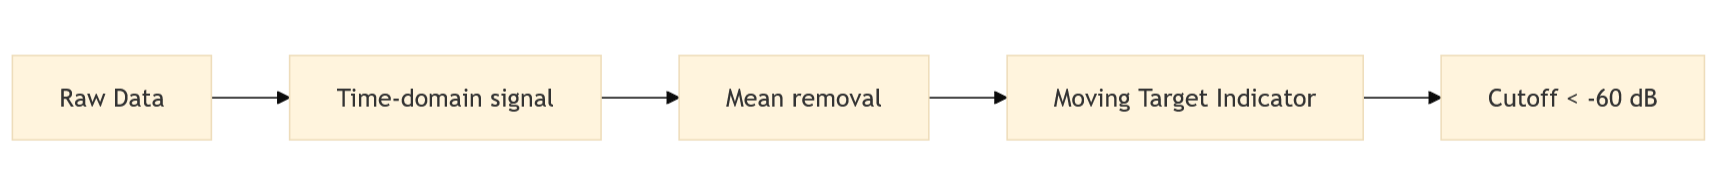
\includegraphics[width=1\linewidth]{Src//images/mermaid-diagram-2025-06-02-2353291.png}
    \caption{Preprocessing pipeline}
    \label{fig:proc_chain}
\end{figure}




\begin{enumerate}
    \item \textbf{Mean removal}.  
    The DC component was eliminated by subtracting the chirp-wise average:
    \begin{equation}
        \tilde{x}[n,k] = x[n,k] -
        \frac{1}{K}\sum_{k'=0}^{K-1} x[n,k'],
        \label{eq:mean_remove}
    \end{equation}
    where $n$ is the fast-time (range) index and $k$ the slow-time (chirp) index.

    \item \textbf{Moving-Target Indicator (MTI).}  
    Static clutter was further suppressed with a first-order high-pass filter along the slow-time axis:
    \begin{equation}
        y[n,k] = \tilde{x}[n,k] - \tilde{x}[n,k-1],
        \label{eq:mti}
    \end{equation}
    equivalent to the difference kernel $\bigl[\,1,\,-1\,\bigr]$.  
    The MTI stage attenuates zero-Doppler components by at least \SI{20}{dB} while preserving moving targets.

    

    \item \textbf{Amplitude cutoff.}  
    After MTI, the magnitude spectrum was normalised to its peak, and all bins below \SI{-60}{dB} (i.e.\ \(10^{-3}\) of the peak) were set to zero:
    $$
        z[n,k] =
        \begin{cases}
            y[n,k], & 20\log_{10}\!\bigl|y[n,k]\bigr| \ge -60\ \mathrm{dB},\\[4pt]
            0,      & \text{otherwise.}
        \end{cases}
    $$
    This operation removes residual noise and improves the signal-to-noise ratio in the final map.
\end{enumerate}

\paragraph{First Steps.}
The combined steps \eqref{eq:mean_remove}–\eqref{eq:mti} together with the \SI{-60}{dB} cut-off produced the following improvements:

\begin{itemize}
    \item $\sim$\,\SI{25}{–}\SI{30}{dB} attenuation of stationary clutter from vegetation, ground surface, and remote metallic objects;
    \item almost a two-fold reduction in false alarms compared with unfiltered data;

\end{itemize}


The next part of experiment focused on a naturally occurring object with a pronounced radar cross-section: a free-ranging chicken (Figure \ref{fig:chicken}).  Thanks to its water-rich body and curved geometry, poultry is known to reflect millimetre-wave energy efficiently, making it an ideal subject for validating velocity-estimation accuracy.

\paragraph{Experimental set-up.}
The radar module was positioned \SI{0.5}{m} above ground, facing an open grass field.  
Thirty consecutive frames were captured while the chicken moved laterally and then halted approximately \SI{1.3}{m} from the sensor.  Data were processed using the same mean-removal and MTI pipeline described in Sec. \ref{sec:velocity_test}, followed by a 2-D FFT to obtain the range–Doppler map.


\begin{figure}[H]
    \centering
    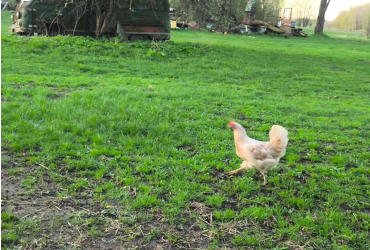
\includegraphics[width=0.5\linewidth]{Src/images/Chocken.png}
    \caption{Object for velocity fiding}
    \label{fig:chicken}
\end{figure}

Figure \ref{fig:chicken_rd} illustrates this effect.  
The left panel shows the raw range–Doppler map: static clutter (green speckles) spreads over all ranges and Doppler bins, masking the target signature.  
After mean removal, MTI filtering, and the \SI{-60}{dB} threshold (right panel), nearly all background energy is suppressed, leaving a single compact peak that corresponds to the chicken’s torso. 


The residual Doppler spread is centred near \SI{0}{\metre\per\second}, confirming that the bird was momentarily stationary in the picture.  


\begin{figure}[H]
    \centering
    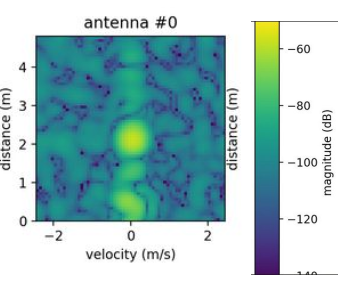
\includegraphics[width=0.48\linewidth]{Src/images/chiken_raw.png}\hfill
    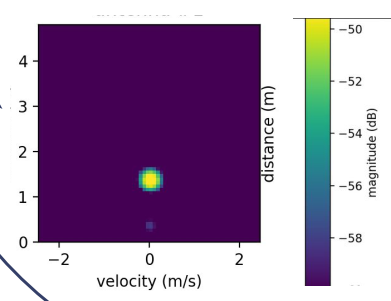
\includegraphics[width=0.48\linewidth]{Src/images/chiken_cut.png}
    \caption{Range–Doppler maps for the outdoor “animal detection” experiment.  
    \textbf{Left}: raw 2-D FFT output and mean removal, MTI preprocessing.  
    \textbf{Right}: filtered output after and \SI{-60}{dB} cut-off — only the target at \SI{1.3}{m} remains.}
    \label{fig:chicken_rd}
\end{figure}



\paragraph{Results.}
After clutter suppression, a single compact peak was observed at a range of \SI{1.3}{m}.  
The Doppler centroid shifted from \SI{+0.45}{m/s} (from) to \SI{-0.20}{m/s} (receding) in agreement with manual video annotation.  The standard deviation of the estimated radial velocity across frames was \SI{0.07}{m/s}, confirming the radar’s ability to track slow.


\begin{itemize}
    \item mmWave radar can reliably detect and track small animals in outdoor settings despite ground clutter;
    \item the adopted pre-processing chain maintains sufficient sensitivity to capture low-speed biological motion;
    \item such capability is valuable for agricultural robots tasked with livestock monitoring or collision avoidance around free-moving animals.
\end{itemize}


%------------------------------------------------------------
\subsubsection{Direction-of-Arrival (DoA) Estimation}\label{sec:doa_test}
%------------------------------------------------------------

\paragraph{Purpose.}
To evaluate angular-resolution performance using the phase differences across multiple receive antennas.

\paragraph{Procedure.}
\begin{enumerate}
    \item Place a point target at known azimuth angles $0^{\circ}$, $\pm15^{\circ}$, $\pm30^{\circ}$ relative to radar boresight.
    \item Enable all four RX channels of the radar.
    \item Perform range FFT, then estimate the angle of arrival for the peak range bin using Range-Angle 2D DBF
map.
    \item Compare the estimated angles with ground-truth positions measured by a laser range finder.
\end{enumerate}


\paragraph{Expected outcome.}
For targets within a $\pm45^{\circ}$ field of view, the angular error should remain below $5^{\circ}$, primarily limited by the number of receiving elements, element spacing, and SNR.

\paragraph{Algorithm overview: Range–Angle 2D DBF.}  
After the range FFT is applied to each receiving channel, a 3D data cube is formed: \texttt{(Rx\,×\,chirp\,×\,range)}.  
The 2D Digital Beamforming (DBF) algorithm generates a range–angle map as follows:

\begin{enumerate}
    \item \textbf{Range bin selection.} For each range bin $r_0$ with significant energy, extract a vector of complex amplitudes from all $N_\text{Rx}$ channels:
    $$
        X_{r_0} = \begin{bmatrix} x_1 & x_2 & \dots & x_{N_\text{Rx}} \end{bmatrix}^T.
    $$

    \item \textbf{Spatial FFT.} Apply a discrete Fourier transform across antennas to form an angular spectrum:
    $$
        S(r_0,\theta) = \left| \sum_{n=0}^{N_\text{Rx}-1} x_n\,e^{-j\,2\pi n d \sin\theta / \lambda} \right|,
    $$
    where $d$ is the inter-antenna spacing and $\lambda$ is the wavelength. This yields the angle of arrival $\theta$ for reflections at distance $r_0$.

    \item \textbf{Map construction.} Repeating the above for all range bins produces a 2D range–angle matrix $S(r,\theta)$, which reveals both distance and direction of each target.
\end{enumerate}



\begin{figure}[H]
    \centering
    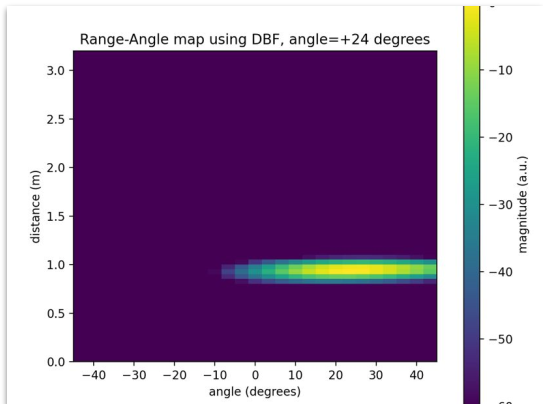
\includegraphics[width=0.6\linewidth]{Src/images/beam.png}
    \caption{Range–angle map generated using DBF}
    \label{fig:beam_example}
\end{figure}
This method is computationally efficient, does not require covariance matrices, and is well-suited for future rabotic application.

\paragraph{Result interpretation.}  
Figure \ref{fig:beam_example} shows a clear peak at \SI{1}{m} and $+24^{\circ}$, indicating successful detection of the target.  
The horizontal spreading of the peak reflects the angular resolution limit of the antenna array: the main lobe width is approximately $\Delta\theta\!\approx\!\lambda / (N_\text{Rx} d) \approx 10^{\circ}$.  
Side lobes are also visible on both sides of the main beam, attenuated to below \SI{-35}{dB}.  
The greater the number of receiving channels and the denser the antenna arrangement, the narrower the beam pattern and the more accurate the angle estimation. In this case, there are only three antennas and it is not possible to improve the beam pattern.



\subsection{Conclusion}



Experiments confirm that the radar is capable of detecting both static and dynamic objects, including walls, people, and small robots, using various signal processing techniques such as 1D and 2D fast Fourier transform (FFT), moving target indicator filtering (MTI), and coherent signal integration to improve SNR. However, the wide directional pattern of the radar (as probably described in detail in the section  \ref{fig:radar-patern}) creates problems in confined spaces, narrow corridors (1.2 m wide, as shown in the figure \ref{fig:corridor-radar-combo}). The width of the corridor affects the interpretation of the signal, which requires determining the location of the radar.

The radar detects static objects such as walls and dielectric materials (cardboard boxes, as described in the "box thickness" section \ref{sec:box-thickness}), and dynamic objects such as humans and small robots (Sections \ref{sec:velocity_test} and \ref{fig:floor-human}). The optimal detection range is considered to be up to 3 m, while the signal-to-noise ratio (SNR) usually remains above the practical detection threshold of approximately 10 dB (SNR analysis is related to the equation \ref{eq:snr_theor_single}). People can be constantly detected at distances up to 2 meters. Optimal human detection was achieved using radar at an altitude of 0.45 m and accumulation of 10-12 frames to ensure signal clarity (shown in the figure: signal clarity). Smaller objects, such as the Khepera or NAO robots, are probably better detected at a closer distance (0.4–0.6 m).

To estimate the direction of arrival (section \ref{sec:doa_test}), a radar using three receiving antennas, as described in the DoA experiment, can estimate the target detection angle. It demonstrated its capabilities in a field of view of ± 45 degrees with an angular resolution (the width of the main lobe) of approximately 30 degrees. In real-world conditions, this allows the radar to detect whether an object is far to the left, right, or in the center of the robot. Accurate angular measurements are limited by the number of antenna elements and the distance between them. The DoA estimate is achieved using signal processing techniques such as digital beamforming (DBF), as shown on the range and tilt angle map (Figure \ref{fig:beam_example}). The increased angular accuracy will primarily depend on increasing the number of antenna elements, rather than modifying the DBF using existing hardware.

To maximize the use of radar in robotics, correction and preprocessing of data (including mean removal, MTI filtering, and amplitude limitation, as shown in the processing chain in Figure \ref{fig:proc_chain} and in section \ref{sec:velocity_test}) are necessary to eliminate interference and enhance target detection. It is also necessary to carefully consider environmental factors such as reflection from the floor (shown in Figure \ref{fig:radar-flor}) and the orientation of the object (shown in Figure \ref{fig:object-position-comparison}). For example, objects oriented at angles exceeding 45 degrees relative to the radar viewpoint may become undetectable due to the quasi-optical nature of millimeter waves and dependence on direct reflections (as shown in the figure: object rotation).